\documentclass[12pt]{article}
\usepackage{amsmath}
\usepackage{bm}
\usepackage{graphicx,psfrag,epsf}
\usepackage{enumerate}
\usepackage{natbib}
\usepackage{url} % not crucial - just used below for the URL 
\usepackage[algo2e]{algorithm2e}
\usepackage{algorithmic}  
\usepackage{algorithm}
\usepackage{mathtools}
\usepackage[toc,page]{appendix}
%\pdfminorversion=4
% NOTE: To produce blinded version, replace "0" with "1" below.
\newcommand{\blind}{0}

% DON'T change margins - should be 1 inch all around.
\addtolength{\oddsidemargin}{-.5in}%
\addtolength{\evensidemargin}{-.5in}%
\addtolength{\textwidth}{1in}%
\addtolength{\textheight}{1.3in}%
\addtolength{\topmargin}{-.8in}%

\DeclarePairedDelimiter\abs{\lvert}{\rvert}
\begin{document}
\def\spacingset#1{\renewcommand{\baselinestretch}%
{#1}\small\normalsize} \spacingset{1}


%%%%%%%%%%%%%%%%%%%%%%%%%%%%%%%%%%%%%%%%%%%%%%%%%%%%%%%%%%%%%%%%%%%%%%%%%%%%%%

\if0\blind
{
  \title{\bf The Hyperedge Event Model}
  \author{Bomin Kim\thanks{
    The authors gratefully acknowledge \textit{please remember to list all relevant funding sources in the unblinded version}}\hspace{.2cm}\\
    Department of Statistics, Pennsylvania State University,\\
  Aaron Schein\\
  College of Information and Computer Sciences, UMass Amherst,\\
    Bruce Desmarais\\
    Department of Political Science, Pennsylvania State University,\\
    and\\
    Hanna Wallach\\
    Microsoft Research NYC}
  \maketitle
} \fi
\if1\blind
{
  \bigskip
  \bigskip
  \bigskip
  \begin{center}
    {\LARGE\bf The Hyperedge Event Model}
\end{center}
  \medskip
} \fi

\bigskip
\begin{abstract}
We introduce the hyperedge event model (HEM)---a generative model for directed edges with multiple recipients or multiple senders. To define the model, we
integrate a dynamic version of the exponential random graph model (ERGM) and generalized linear model (GLM) approach to jointly understand who communicates with whom, and when. We use the model to analyze emails sent between department managers in Montgomery county government in North Carolina. Our application demonstrates that the model is effective at predicting and explaining time-stamped network data involving edges with multiple recipients.
	\end{abstract}

\noindent%
{\it Keywords:}  3 to 6 keywords, that do not appear in the title
\vfill

\newpage
\spacingset{1.45} % DON'T change the spacing!
\section{Introduction}\label{sec:intro}
In recent decades, real-time digitized textual communication has developed into a ubiquitous form of social and professional interaction \citep{kanungo2008modeling, szostek2011dealing, burgess2004email, pew2016}. From the perspective of the computational social scientist, this has led to a growing need for methods of modeling interactions that manifest as edges exchanged in continuous time. A number of models that build upon topic modeling through Latent Dirichlet Allocation \citep{Blei2003} to incorporate link data as well as textual content have been developed recently \citep{mccallum2005author,lim2013twitter,Krafft2012}. These models are innovative in their extensions that incorporate network information. However, none of the models that are currently available in the literature integrate the rich random-graph structure offered by state of the art models for network structure---such as the exponential random graph model (ERGM) \citep{robins2007introduction,chatterjee2013estimating,hunter2008ergm}. The ERGM is the canonical model for modeling the structure of a static network. It is flexible enough to specify a generative model that accounts for nearly any pattern of edge formation such as reciprocity, clustering, popularity effects \citep{desmarais2017statistical}. 

Several network models have been developed that handle time-stamped events in which edge formation is governed by structural dynamics similar to those used in the ERGM \citep{Butts2008,Vu2011,snijders1996stochastic}. Those models are very useful to understand which traits and behaviours are predictive of interactions, however, none of the models explicitly allows hyperedges---a connection between two or more vertices generated simultaneously\footnote{A hyperedge connecting just two nodes is simply a usual dyadic edge.}---which is a common property of digitalized textual interactions such as emails and online messages. For instance, \cite{PerryWolfe2012} treat multicast interactions---one type of directed hyperedge which involve one sender and multiple receivers---via duplication (i.e., obtain pairwise interactions from the original multicast), but their model parameter estimation relies on likelihood approximation which leads to bias. Similarly, \cite{fan2009learning} treats multicast emails as multiple single-recipient edges and randomly jitter the sent times, to avoid the violation of continous-time model assumption. On the other hand, there have been numerous studies for hyperedges under the hypergraph theory \citep{karypis1999multilevel} in phyics literature, including a random hypergraph model \citep{ghoshal2009random}, but most of them are designed specifically for engineering applications---e.g., multiple tagging networks \citep{zlatic2009hypergraph,zhang2010hypergraph}, cellular networks \citep{klamt2009hypergraphs}, and personalized recommendations \citep{zhang2010personalized,blattner2009b}. To our knowledge, there is a lack of extensive efforts to incorportate hyperedge modeling into general statistical framework.

Concentrating on developing a statistical network model with better handling of hyperedges, we introduce the hyperedge event model (HEM) which simultaneously models the two components that govern time-stamped event formation: 1) the recipient selection processs that allows multiple senders or receivers, and 2) the time-to-next interactions with flexible distributional choices. In what follows, we introduce the HEM by describing how we assume the generatve process of a time-stamped event data (Section 2), and deriving the sampling equations for Bayesian inference (Section 3). Then, we apply the model to the Montgomery county government email data and perform two model validation tasks (Section 4). Finally, the paper finishes in Section 5 with conclusion and discussion.

\section{The Hyperedge Event Model (HEM)}\label{sec:generative process}
Data generated under the model consists of $D$ unique edges. A single edge, indexed by $d \in [D]$, is represented by the three components: the sender $a_d \in [A]$, an indicator vector of recipients $\boldsymbol{r}_d = \{u_{dr} \}_{r=1}^{A}$, and the timestamp $t_d \in (0, \infty)$. For simplicity, we assume that edges are ordered by time such that $t_d \leq t_{d+1}$. While the model can be applied for two type of hyperedges---edges with (1) a single sender and multiple receivers, and (2) multiple senders and a single receiver---here we only present the generative process for those involving a single sender and multiple receivers (i.e., multicast). For the latter case of hyperedges, we treat $a_d$ to be an indicator vector of senders $\boldsymbol{a}_d = \{u_{dr} \}_{a=1}^{A}$ and $r_d$ to be the single recipient.
\subsection{Edge Generating Process}\label{subsec: Tie}
For every possible author--recipient pair $(a,r)_{a \neq r}$, we define the ``recipient intensity", which is the likelihood of edge $d$ being sent from $a$ to $r$:
\begin{equation}
\lambda_{adr} = {\boldsymbol{b}}^{\top}\boldsymbol{x}_{adr},
\end{equation}
where $\boldsymbol{b}$ is $P$--dimensional vector of coefficients and $\boldsymbol{x}_{adr}$ is a set of network features which vary depending on the hypotheses regarding canonical processes relevant to network theory such as popularity, reciprocity, and transitivity. In addition, we include intercept term to account for the average (or baseline) number of recipients. We place a Normal prior $\boldsymbol{b} \sim N(\boldsymbol{\mu}_b, \Sigma_b)$.

Next, we hypothesize ``If $a$ were the sender of edge $d$, who would be the recipient(s)?" To do this, we draw each sender's set of recipients from the multivariate Bernoulli (MB) distribution \citep{dai2013multivariate}---a model to estimate the structure of graphs with binary nodes---with probability of 1 being logit($\lambda_{adr}$). In order to avoid the model degeneracy from having an empty recipient set, we define a probability measure ``MB$_{G}$" motivated by the non-empty Gibbs measure \citep{fellows2017removing} which excludes the all-zero vector from the support of the multivariabe Bernoulli distirbution. As a result, we 1) allow multiple recipients or ``multicast", 2) prevent from obtaining zero recipient, and 3) ensure tractable normalizing constant. To be specific, we draw a binary vector $\boldsymbol{u}_{ad}= (u_{ad1},
\ldots, u_{adA})$ 
\begin{equation} \boldsymbol{u}_{ad}  \sim
\mbox{MB}_{G}(\boldsymbol{\lambda}_{ad}),
\end{equation}
where $\boldsymbol{\lambda}_{id}= \{\lambda_{adr}\}_{r=1}^A$. In particular, we define $\mbox{MB}_{G}(\boldsymbol{\lambda}_{ad})$ as
\begin{equation}
\begin{aligned}
&p(\boldsymbol{u}_{ad}|\delta, \boldsymbol{\lambda}_{ad}) = \frac{\exp\Big\{\mbox{log}\big(\text{I}( \lVert \boldsymbol{u}_{ad}\rVert_1 > 0 )\big) + \sum_{r\neq a} \lambda_{adr}u_{adr}\Big\}}{Z(\boldsymbol{\lambda}_{ad})} ,
\end{aligned}
\label{eqn:Gibbs}
\end{equation}
where $Z(\boldsymbol{\lambda}_{ad})= \prod_{r \neq a} \big(\mbox{exp}(\lambda_{adr}) + 1\big)-1$ is the normalizing constant and $\lVert \cdot \rVert_1$ is the $l_1$--norm. Again, this is equivalent to assume independent Bernoulli trial on each $u_{adr}$ with probability of 1 being logit($\lambda_{adr}$), excluding the case when all $u_{adr}=0$. We provide the derivation of the normalizing constant as a tractable form in the supplementary material. 


\subsection{Time Generating Process}\label{subsec:Time}
Similarly, we hypothesize ``If $a$ were the sender of edge $d$, when would it be sent?" and define the ``timing rate" for sender $a$
\begin{equation}
\mu_{ad} = g^{-1}(\boldsymbol{\eta}^\top \boldsymbol{y}_{ad}),
\end{equation}
where $\boldsymbol{\eta}$ is $Q$--dimensional vector of coefficients with a Normal prior $\boldsymbol{\eta} \sim N(\boldsymbol{\mu}_\eta,\Sigma_\eta)$, $\boldsymbol{y}_{ad}$ is a set of time-related covariates, e.g., any feature that could affect timestamps of the edge, and $g(\cdot)$ is the appropriate link function such as identity, log, or inverse. 

In modeling ``when", we do not directly model the timestamp $t_d$. Instead, we assume that each sender's the time-increment or ``time to next interaction" (i.e., $\tau_{d} = t_d-t_{d-1}$) is drawn from a specific distribution in the exponential family.  We follow the generalized linear model (GLM) framework \citep{nelder1972generalized}:
\begin{equation}
\begin{aligned}
E(\tau_{ad}) &= \mu_{ad},\\
V(\tau_{ad}) &= V(\mu_{ad}),
\end{aligned}
\end{equation}
where $\tau_{ad}$ here is a positive real number. Possible choices of distribution include exponential, Weibull, gamma, and lognormal\footnote{lognormal distribution is not exponential family but can be used via modeling of $\log(\tau_d)$.} distributions, which are commonly used in time-to-event modeling \citep{rao2000applied,rizopoulos2012joint}. Based on the choice of distribution, we may introduce any additional parameter (e.g., $\sigma_\tau^2$) to account for the variance. We use $f_\tau(\cdot; \mu, \sigma_\tau^2)$ and $F_\tau(\cdot; \mu, \sigma_\tau^2)$ to denote the probability density function (p.d.f) and cumulative density function (c.d.f), respectively, with mean $\mu$ and variance $\sigma^2$.

\subsection{Observed Data}\label{subsec:Observed}
Finally, we choose the sender, recipients, and timestamp---which will be observed---by selecting the sender--recipient-set pair with the smallest time-increment \citep{snijders1996stochastic}:
\begin{equation}
\begin{aligned}
a_d &= \mbox{argmin}_{a}(\tau_{ad}),\\
\boldsymbol{r}_d &= \boldsymbol{u}_{a_d d},\\
t_d &=t_{d-1} + \tau_{a_d d}.
\end{aligned}
\end{equation}
Therefore, it is a sender-driven process in that the recipients and timestamp of an edge is determined by the sender's urgency to send the edge to chosen recipients. Note that  our generative process accounts for tied events such that in case of tied events (i.e., multiple senders generated exactly same time increments $\tau_d$), we observe all of the tied events without assigning the orders of tied events. Algorithm \ref{alg:generative} summarizes the generative process in Section \ref{sec:generative process}.
	\begin{algorithm}[ht]
		\spacingset{1}
		\SetAlgoLined
		\caption{Generating Process}
		\For{d=1 to D}{
			\For{a=1 to $A$}{
				\For{r=1 to $A$ (r $\neq$ a)}{
						set $\lambda_{adr} = {\boldsymbol{b}}^{\top}\boldsymbol{x}_{adr}$
					}  
					draw $\boldsymbol{u}_{ad}  \sim
					\mbox{Gibbs}(\boldsymbol{\lambda}_{ad})$\\
					set $\mu_{ad} = g^{-1}(\boldsymbol{\eta}^\top \boldsymbol{y}_{ad})$\\
					draw $\tau_{ad} \sim f_\tau(\mu_{ad}, \sigma_\tau^2)$
				}
				\textbf{For no tied events,}\\
				set $a_d= \mbox{argmin}_{a}(\tau_{ad})$\\
				set $\boldsymbol{r}_d = \boldsymbol{u}_{a_d d}$\\
				set $t_d =t_{d-1} + \min_a\tau_{ad}$\\\\
				\textbf{For $n$ tied events,} (i.e., $n$ senders generated same minimum time increments)\\
				set $a_d, \ldots, a_{d+n}= \mbox{argmin}_{a}(\tau_{ad})$\\
				set $\boldsymbol{r}_d=\boldsymbol{u}_{a_d d},\ldots,\boldsymbol{r}_{d+n}= ,\boldsymbol{u}_{a_{d+n} d}$\\
				set $t_d, \ldots, t_{d+n}=t_{d-1} + \min_a\tau_{ad}$\\
				jump to $d = d+n+1$
			}
			\label{alg:generative}
		\end{algorithm}
\spacingset{1.45}
\section{Posterior Inference}\label{sec:inference}
Our inference goal is to invert the generative process to obtain the posterior distribution over the unknown parameters, conditioned on the observed data and hyperparamters $(\boldsymbol{\mu}_b, \Sigma_b, \boldsymbol{\mu}_\eta, \Sigma_\eta)$. We draw the samples using Markov chain Monte Carlo (MCMC) methods, repeatedly resampling the value of each parameter from its conditional posterior given the observed data, hyperparamters, and the current values of the other parameters. We express each parameter’s conditional posterior in a closed form using the data augmentation schemes in $\boldsymbol{u}$ \citep{tanner1987calculation}. In this section, we provide each latent variable's conditional posterior. 

First, since $u_{adr}$ is a binary random variable, new values may be sampled directly using
\begin{equation}
\begin{aligned}
&P(u_{adr}=1| \boldsymbol{u}_{ad\backslash r}, \boldsymbol{b}, \boldsymbol{x})
\propto \mbox{exp}(\lambda_{adr});\\
&P(u_{adr}=0| \boldsymbol{u}_{ad\backslash r},\boldsymbol{b}, \boldsymbol{x})\propto \text{I}(\lVert\boldsymbol{u}_{ad\backslash r}\rVert_1 > 0 ),
\end{aligned}
\label{eqn:latentreceiver}
\end{equation}
where $I(\cdot)$ is the indicator function that is used to prevent from the instances where a sender chooses zero number of recipients.

New values for continuous variables $\boldsymbol{b},$ and $\boldsymbol{\eta}$ and $\sigma^2_\tau$ (if applicable) cannot be sampled directly from their conditional posteriors, but may instead be obtained using the Metropolis--Hastings algorithm. With uninformative priors (i.e., $N({0},\infty)$), the conditional posterior over $\boldsymbol{b}$ is
\begin{equation}
P(\boldsymbol{b}| \boldsymbol{u}, \boldsymbol{x})\propto \prod_{d=1}^D
\prod_{a=1}^A \frac{\exp\Big\{\mbox{log}\big(\text{I}( \lVert \boldsymbol{u}_{ad}\rVert_1 > 0)\big) + \sum\limits_{r \neq a} \lambda_{adr}u_{adr}\Big\}}{Z(\boldsymbol{\lambda}_{ad})},
\end{equation}
where the two variables share the conditional posterior and thus can be jointly sampled. Likewise, assuming uninformative priors on $\boldsymbol{\eta}$ (i.e., $N({0},\infty)$) and $\sigma_{\tau}^2$ (i.e., half-Cauchy($\infty$)), the conditional posterior for no-tied event case is
\begin{equation}
P(\boldsymbol{\eta}, \sigma_\tau^2| \boldsymbol{u}, \boldsymbol{y})\propto \prod_{d=1}^D\Big(f_{\tau}(\tau_{d}; \mu_{a_d d}, \sigma_\tau^2)\times \prod_{a\neq a_d}\big(1-F_{\tau}(\tau_{d}; \mu_{a d}, \sigma_\tau^2) \big)\Big),
\end{equation}
where $f_{\tau}(\tau_{d}; \mu_{a_d d}, \sigma_\tau^2)$ is the probability that the $d^{th}$ observed time-increment comes from the specified distribution $f_\tau(\cdot)$ with the observed sender's mean parameter, and $\prod_{a\neq a_d}\big(1-F_{\tau}(\tau_{d}; \mu_{a d}, \sigma_\tau^2) \big)$ is the probability that the latent (or unobserved) senders for event $d$ all generated time-increments greater than $\tau_d$. Moreover, under the existence of tied-event, the conditional posterior of $\boldsymbol{\eta}$ and $\sigma_{\tau}^2$ should be written as
\begin{equation}
\begin{aligned}
&P(\boldsymbol{\eta}, \sigma_\tau^2| \boldsymbol{u}, \boldsymbol{y})\\&\propto \prod_{m=1}^M\Big(\prod_{d:t_d=t_m^*}f_{\tau}(t_m^*-t_{m-1}^*; \mu_{a_d d}, \sigma_\tau^2)\times \prod_{a \notin \{a_d\}_{d:t_d=t_m^*}}\big(1-F_{\tau}(t_m^*-t_{m-1}^*; \mu_{a d}, \sigma_\tau^2) \big)\Big),
\end{aligned}
\end{equation}
where $t_1^*,\ldots,t_M^*$ are the unique timepoints across $D$ events ($M \leq D$). If $M=D$ (i.e., no tied events), Equation (10) reduces to Equation (9). Algorithm \ref{alg:MCMC} provides the pseudocode.
 \begin{algorithm}[H]
 			\spacingset{1}
 	\SetAlgoLined
 	\caption{MCMC Algorithm}
 	set initial values of $\boldsymbol{b}, \boldsymbol{\eta}$, (and $\sigma_\tau^2$)\\
 	\For{o=1 to outer}{
 	 		\For{d=1 to D}{
 			\For{a = 1 to A}{
 				\For{r = 1 to A (r $\neq$ a)}{
 						update $u_{adr}$ using Gibbs update --- Equation (7)
	 			}
 			}
 		}
 		 		\For{n=1 to inner1}{
 		 			update $\boldsymbol{b}$ using Metropolis-Hastings --- Equation (8)
 				}
 		\For{n=1 to inner2}{
 				update $\boldsymbol{\eta}$ using Metropolis-Hastings --- Equation (10)\\
 				(if needed) update $\sigma_\tau^2$ using Metropolis-Hastings --- Equation (10)
 		}
 }
 	Summarize the results with: last chain of $\boldsymbol{b}$, and last chain of $\boldsymbol{\eta}$ (and $\sigma_\tau^2$) 
 				\label{alg:MCMC}
 \end{algorithm}
 	   \section{Application to Montgomary County Emails}\label{subsec:Emails}
 	  We now present a case study applying our method to Montgomery county government email data. For this case study,
 	  we formulate the network statistics $\boldsymbol{x}$ and timestamp statistics $\boldsymbol{y}$ and ground them in illustrative examples. We then report a suite of experiments that test our method’s ability to form the posterior distribution over latent variables. 
 	  	   \subsection{Data}\label{subsec:Montgomery}
 	   Our data come from the North Carolina county government email dataset collected by \cite{ben2017transparency} that includes internal email corpora covering the inboxes and outboxes of managerial-level employees of North Carolina county governments. Out of over twenty counties, we chose Montgomery County to 1) test our model using data with a lot of hyperedges (16.76\%), all of which are a single sender multiple receiver cases, and 2) limit the scope of this initial application. To summarize, Montgomery County email network contains 680 emails, sent and received by 18 department managers over a period of 3 months (March--May) in 2012. 
 	   \subsection{Covariates}\label{subsec:Covariates_email}
	In the example of email networks, we form the covariate vector $\boldsymbol{x}_{adr}$ using time-varying network statistics based on the time interval prior to and including $t_{d-1}$. Given a set of interaction data, a primary modeling goal lies in determining which characteristics and behaviors of the senders and receivers are predictive of interaction. This email application specifically give rise to the following question: ``To what extent are nodal, dyadic or triadic network effects, as characterized
by past interaction behaviors, relevant to predicting future events?" We employ the network statistics in \cite{PerryWolfe2012}, along with the intercept term, to address the question. Specifically, our time interval tracks 7 days prior to the last email was sent $l_d = (t_{d-1}-7\mbox{ days}, t_{d-1}]$. For $a \in [A], r \in [A]$, and $d \in [D]$, we define the effects
	\begin{itemize}
		\spacingset{1}
		\item[1.] intercept: ${x}_{adr1} =1$;
		\item[2.] outdegree of sender $a$: ${x}_{adr2} =\sum_{d^\prime: t_{d^\prime} \in l_d} I(a_{d^\prime} = a)$;
		\item[3.] indegree of receiver $r$: ${x}_{adr3}=\sum_{d^\prime: t_{d^\prime} \in l_d} I(u_{d^\prime r} = 1)$;
		\item[4.] send: ${x}_{adr4}=\sum_{d^\prime: t_{d^\prime} \in l_d} I(a_{d^\prime} = a)I(u_{d^\prime r} = 1)$;
		\item[5.] receive: ${x}_{adr5}=\mbox{send}(r,a)$;
		\item[6.] 2-send: ${x}_{adr6} = \sum_{h \neq a, r} \mbox{send}(a,h)\mbox{send}(h,r)$;
		\item[7.] 2-receive: ${x}_{adr7}= \sum_{h \neq a, r} \mbox{send}(h,a)\mbox{send}(r,h)$;
		\item[8.] sibling: ${x}_{adr8}=\sum_{h \neq a, r} \mbox{send}(h,a)\mbox{send}(h,r)$;
		\item[9.] cosibling: ${x}_{adr9}=\sum_{h \neq a, r} \mbox{send}(a,h)\mbox{send}(r,h)$;
		\item[10.] hyperedge size of sender $a$: ${x}_{adr10}=\sum_{d^\prime: t_{d^\prime} \in l_d} \sum_{r=1}^A I(a_{d^\prime} = a)I(u_{d^\prime r} = 1)$;
		\item[11.] outdegree$*$hyperedge size: ${x}_{adr11} = {x}_{adr2}\times{x}_{adr10};$
	\end{itemize}
	where $I(\cdot)$ is an indicator function, and the last covariate is the interaction term between outdegree and hyperedge size. As with the nodal (2, 3, 10, 11) and dyadic (4, 5) effects, the triadic (6--9) effects are designed so that their coefficient have a straightforward interpretation. Dyadic statistics ``send" and ``receive" are defined as above such that these covariates measure the number of emails sent from $a$ to $r$ and $r$ to $a$, respectively, within the last 7 days. In the example of triadic statistics, the covariate ``2-send" counts the pairs of emails involving some node $h$ distinct from $a$ and $r$ such that an email from $a$ to $h$ and $h$ to $r$ are separately observed within the last 7 days. Other triadic covariates behave similarly, and their interpretations are also analogous, which are illustrated in Figure \ref{figure:netstats}.
		\begin{figure}[!t]
			\centering
			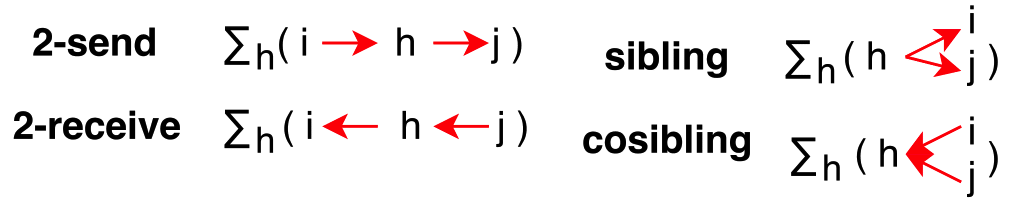
\includegraphics[width=0.55\textwidth]{plots_paper/triad.png}	
			\caption {Visualization of triadic statistics.}
			\label{figure:netstats}
		\end{figure}

For time-related covariates $\boldsymbol{y}_{ad}$ in Section \ref{subsec:Time}, we form the covariate vector $\boldsymbol{y}_{ad}$ using the seven statistics which may possibly effect ``time to send the next document". Note that these statistics could depend on $a$ only (nodal effect), $d$ (or $t_d$) only (temporal effect), or both $a$ and $d$ (nodal \& temporal effect). Specifically, the statistics are defined as
\begin{itemize}
	\spacingset{1}
	\item[1.] intercept: ${y}_{ad1} =1$;
	\item[2.] outdegree of sender $a$: ${y}_{ad2} =\sum_{d^\prime: t_{d^\prime} \in l_d} I(a_{d^\prime} = a)$;
	\item[3.] indegree of sender $a$: ${y}_{ad3}=\sum_{d^\prime: t_{d^\prime} \in l_d} I(u_{d^\prime a} = 1)$;
	\item[4.] gender of sender $a$: ${y}_{ad4}=I(a= \mbox{female})$;
	\item[5.] manager status of sender $a$: ${y}_{ad5}=I(a= \mbox{County Manager})$;
	\item[6.] weekend of event $d$: ${y}_{ad6} = I(t_{d-1}= \mbox{weekend})$;
	\item[7.] am/pm of event $d$: ${y}_{ad7}= I(t_{d-1}= \mbox{pm})$.
\end{itemize}

	\subsection{Prediction Experiment}\label{subsec:Experiment_email}
	
	The HEM has many component parts that need to be specified by the user (i.e., the selection of the event timing features $\bm{y}$, the recipient selection features $\bm{x}$, and the event time distribution $f$). Many of these components will be specified based on user expertise (e.g., regarding which features would drive recipient selection), but some decisions may require a data-driven approach to model specification. For example, though theoretical considerations may inform the specification of features, subject-matter expertise is unlikely to inform the decision regarding the family of the event time distribution. Furthermore, since different distribution families (and model specifications more generally) may involve different size parameter spaces, any data-driven approach to model comparison must guard against over-fitting the data. In this section we present a general-purpose approach to evaluating the HEM specification using out-of-sample prediction. We illustrate this approach by comparing alternative distributional families for the event timing component of the model. Here, we specifically compare the predictive performance from two distributions---lognormal and exponential. We particularly choose exponential distribution as an alternative to what we used earlier (i.e., lognormal) since exponential is the most commonly specified distribution for time-to-event data which is also used in the stochastic actor oriented models \citep{snijders1996stochastic} as well as their extensions \citep{snijders2007modeling}. 

		We evaluate the model's ability to predict edges and timestamps from the Montgomery County email data, conditioned on their ``training" part of the data. To perform the experiment, we separately formed a test split of each three components---sender, recipients, and timestamps---by randomly selecting ``test" data with probability $p=0.1$. Any missing variables were imputed by drawing samples from their conditional posterior distributions, given the observed data, parameter estimates, and current values of test data. We then run inference to update the latent variables given the imputed and observed data. We iterate the two steps---imputation and inference---multiple times to obtain enough number of estimates for ``test" data. Algorithm \ref{alg:PPE} outlines this procedure in detail. We run the experiment and measure the predictive performance of two separate time distributions using 500 predicted samples, which are depicted in Figure \ref{figure:PPEresults}. First, we compare the correct sender probability for missing documents $\{d:a_d=\mbox{NA}\}$, which corresponds to $\pi_{a_{d}}=P(a_{d} = a^{obs}_{d}|\cdot)$ in Algorithm \ref{alg:PPE}. The plot on the left shows that lognormal distribution reaches higher correct sender probability than exponential distribution, although their centers (e.g., medians) are similar. Secondly, we compute similar measure for recipients---correct recipient probability $P(r_{dr} = r^{obs}_{dr})$ in Algorithm \ref{alg:PPE} where $r^{obs}_{dr}$ is either 1 (received) or 0 (not received)---and visually compare the two distributions in logit scale (i.e., $\log(\frac{P(r_{dr} = r^{obs}_{dr}|\cdot)}{1-P(r_{dr} = r^{obs}_{dr})})$). Since the edge generating process (Section \ref{subsec: Tie}) is not directly affected by the choice of timestamp distribution, there is no significant difference between lognormal and exponential in their performance of predicting unknown recipients. Finally, prediction errors for missing timestamps are measured using the median absolute percentage error (MdAPE) \citep{hyndman2006another}, where we take the median of absolute percentage errors $p_{di}$ for $i=1,\ldots,500$ for $d$th document, calculated as follows:
		\begin{algorithm}[!t]
			\spacingset{1}
			\caption{Out-of-Sample Predictions}
			\label{alg:PPE}
			\begin{algorithmic}
				\STATE {\bfseries Input:} data $ \{ (a_d, \boldsymbol{r}_d, t_d)\}_{d=1}^D$, 
				number of new data to generate $R$,
				hyperparameters
				\vskip 0.1in
				\textbf{Test splits:}	
				\STATE draw test authors with $p=0.1$ (out of $D$ authors) 
				\STATE draw test recipients
				with $p=0.1$ (out of $D\times (A-1)$ recipient indicators $\{\{\boldsymbol{r}_{dr}\}_{r\in [A]_{\backslash a_d}}\}_{d=1}^D$)
				\STATE draw test timestamps with $p=0.1$  (out of $D$ timestamps) 
				\STATE set the ``test" data as ``missing" (NA)
				\vskip 0.1in
				\textbf{Imputation and inference:}	
				\STATE initialize the parameters $(\boldsymbol{b}, \boldsymbol{\eta}, \boldsymbol{u}, \sigma^2_\tau)$
				\FOR{$r=1$ {\bfseries to}  $R$}
				\FOR{$d=1$ {\bfseries to}  $D$}
				\IF{$a_d=$  NA}
				\FOR{$a=1$ {\bfseries to} $A$}
				\STATE compute $\pi_{a} $ using $P(a_d= a | \cdot)=f_{\tau}(\tau_{d}; \mu_{a_dd}, \sigma_\tau^2)\times \prod_{a\neq a_d}\big(1-F_{\tau}(\tau_{d}; \mu_{a d}, \sigma_\tau^2) \big)$
				\ENDFOR
				\STATE draw $a_d \sim \mbox{Multinomial}(\pi_a)$
				\ENDIF
				\FOR{$r\in [A]_{\backslash a_d}$}
				\IF{$r_{dr}=$ NA}
				\STATE draw $r_{dr}$ using $P(r_{dr}= 1 | \cdot)$ and $P(r_{dr}= 0| \cdot)$---Equation (7)
				\ENDIF
				\ENDFOR
				\IF{$t_d=$ NA}
				\STATE draw $\boldsymbol{\tau}^{new}_d$ from $f_{\tau}(\tau^{new}_{d}; \mu_{a_d d}, \sigma_\tau^2)\times \prod_{a\neq a_d}\big(1-F_{\tau}(\tau_{d}; \mu_{a d}, \sigma_\tau^2) \big)$ via importance sampling (e.g., proposal distribution $g \sim \mbox{halfcauchy}(5)$)
				\ENDIF
				\STATE run inference and update $(\boldsymbol{b}, \boldsymbol{\eta},\boldsymbol{u}, \sigma^2_\tau)$ given the imputed and observed data
				\ENDFOR
				\STATE store the estimates for ``test" data
				\ENDFOR
			\end{algorithmic}
		\end{algorithm}
	\begin{figure}[!t]
		\centering
		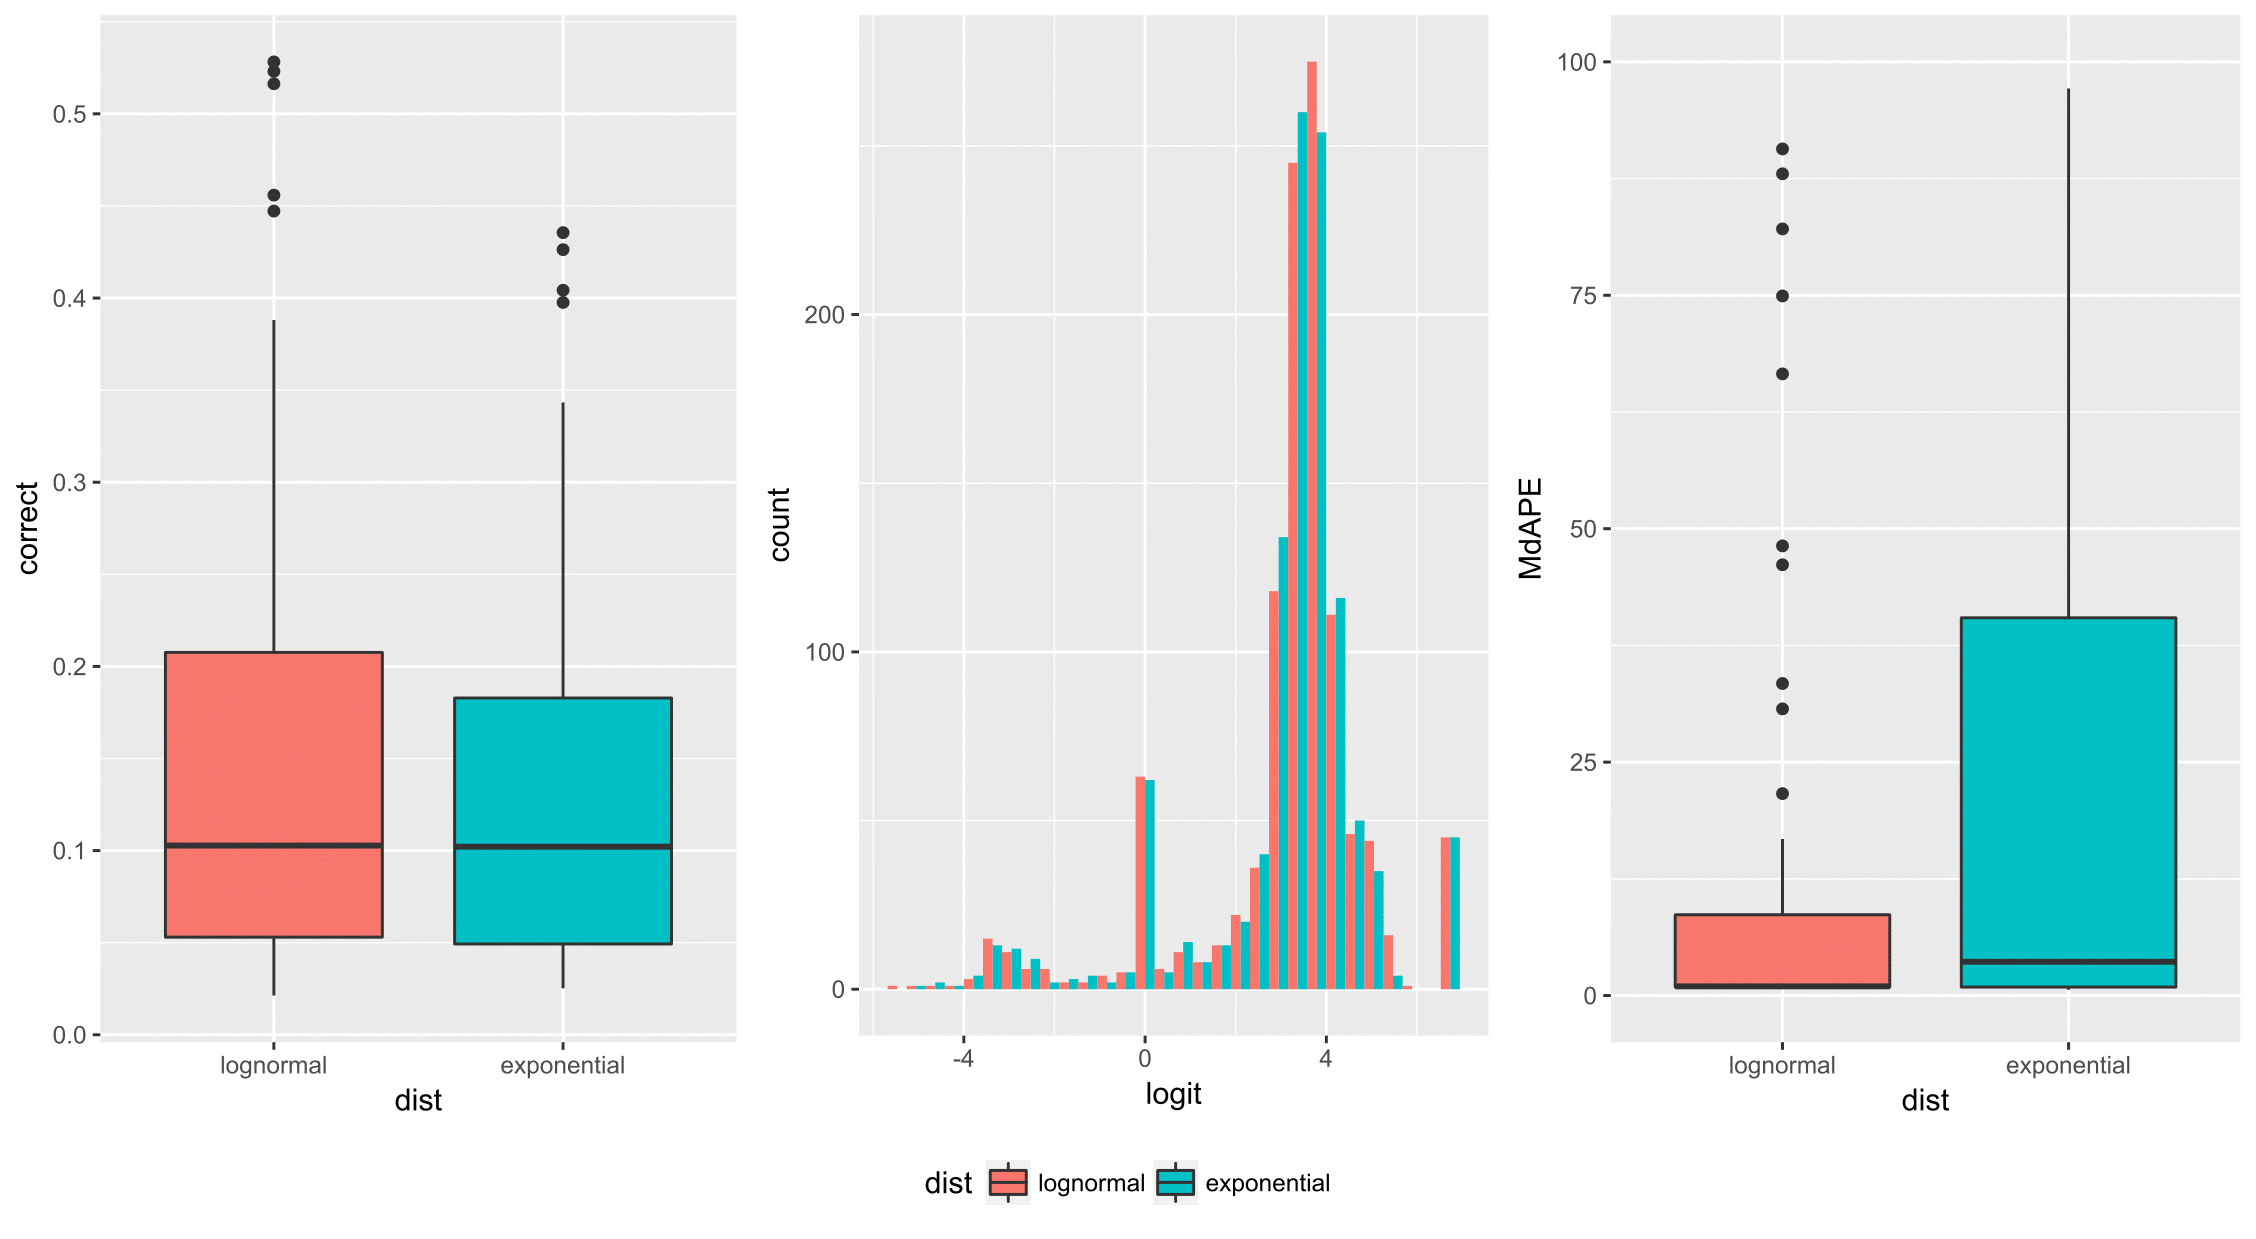
\includegraphics[width=1\textwidth]{plots_paper/PPEplot-1.png}	
		\caption {Comparison of predictive performance between lognormal and exponential distributions: boxplots for correct sender probability (\textit{left}), distribution of correct recipient probability in logit (\textit{middle}), and boxplots for median absolute percentage error (\textit{right}).}
		\label{figure:PPEresults}
	\end{figure}
	\begin{equation*}
	p_{di} = \abs*{\frac{\tau^{obs}_d - \tau^{pred}_{di}}{\tau^{obs}_d}},
	\end{equation*}
	and we present boxplots for the MdAPE estimates on the right plot. As expected, we have huge benefit in the performance of timestamp prediction when we choose lognormal distribution over exponential. This difference can be explained by our variance estimate $\hat{\sigma}_\tau^2= 14.093$ in Section \ref{subsec:Result_email}, because exponential distribution omits the extra information on time-increments contained in the large variance estimate. As illustrated above, we can use this out-of-sample prediction task for two usage---1) provide an effective answer to the question ``how are we filling in the missing information of the emails?" and 2) offer one standard way to determine the time-increment distribution in Section \ref{subsec:Time}. 
	\subsection{Posterior Predictive Checks}\label{subsec:PPC_email} 	   
	We perform posterior predictive checks \citep{rubin1984bayesianly} to evaluate the appropriateness of our model specification for the Montgomery County email data. We formally generated entirely new data, by simulating time-stamped events $\{(a_{d}, \boldsymbol{r}_{d}, t_{d})\}_{d=1}^D$ from the genenerative process in Section \ref{sec:generative process}, conditional upon a set of inferred parameter values from the inference in Section \ref{subsec:Result_email}. For the test of goodness-of-fit in terms of network dynamics, we use multiple network statistics that summarize meaningful aspects of the Montgomery County email data: outdegree distribution, indegree distribution, recipient size distribution, and time-increments probability-probability (PP) plot. We then generated 500 synthetic networks from the posterior predictive distribution, according to Algorithm \ref{alg:PPC}.
	\begin{algorithm}[!b]
		\spacingset{1}
		\caption{Generate new data for PPC}
		\begin{algorithmic}
			\STATE \textbf{Input}: number of new data to generate $R$, covariates $\boldsymbol{x}$ and $\boldsymbol{y}$\\
			estimated latent variables $(\boldsymbol{u}, \boldsymbol{b}, \boldsymbol{\eta},  \sigma_\tau^2)$\\
			\vskip 0.1in
			
			\FOR{$r=1$ {\bfseries to}  $R$}
			\FOR{$d = 1$ {\bfseries to}  $D$} 
			\STATE	Draw ($a_{d}$, $\boldsymbol{r}_{d}$, $t_{d}$) following Section \ref{sec:generative process}\\
			\ENDFOR
			\STATE Store every $r^{th}$ new data $\{(a_{d}, \boldsymbol{r}_{d}, t_{d})\}_{d=1}^D$ 
			\ENDFOR
		\end{algorithmic}
		\label{alg:PPC}
	\end{algorithm}       
	\begin{figure}[!t]
		\centering
		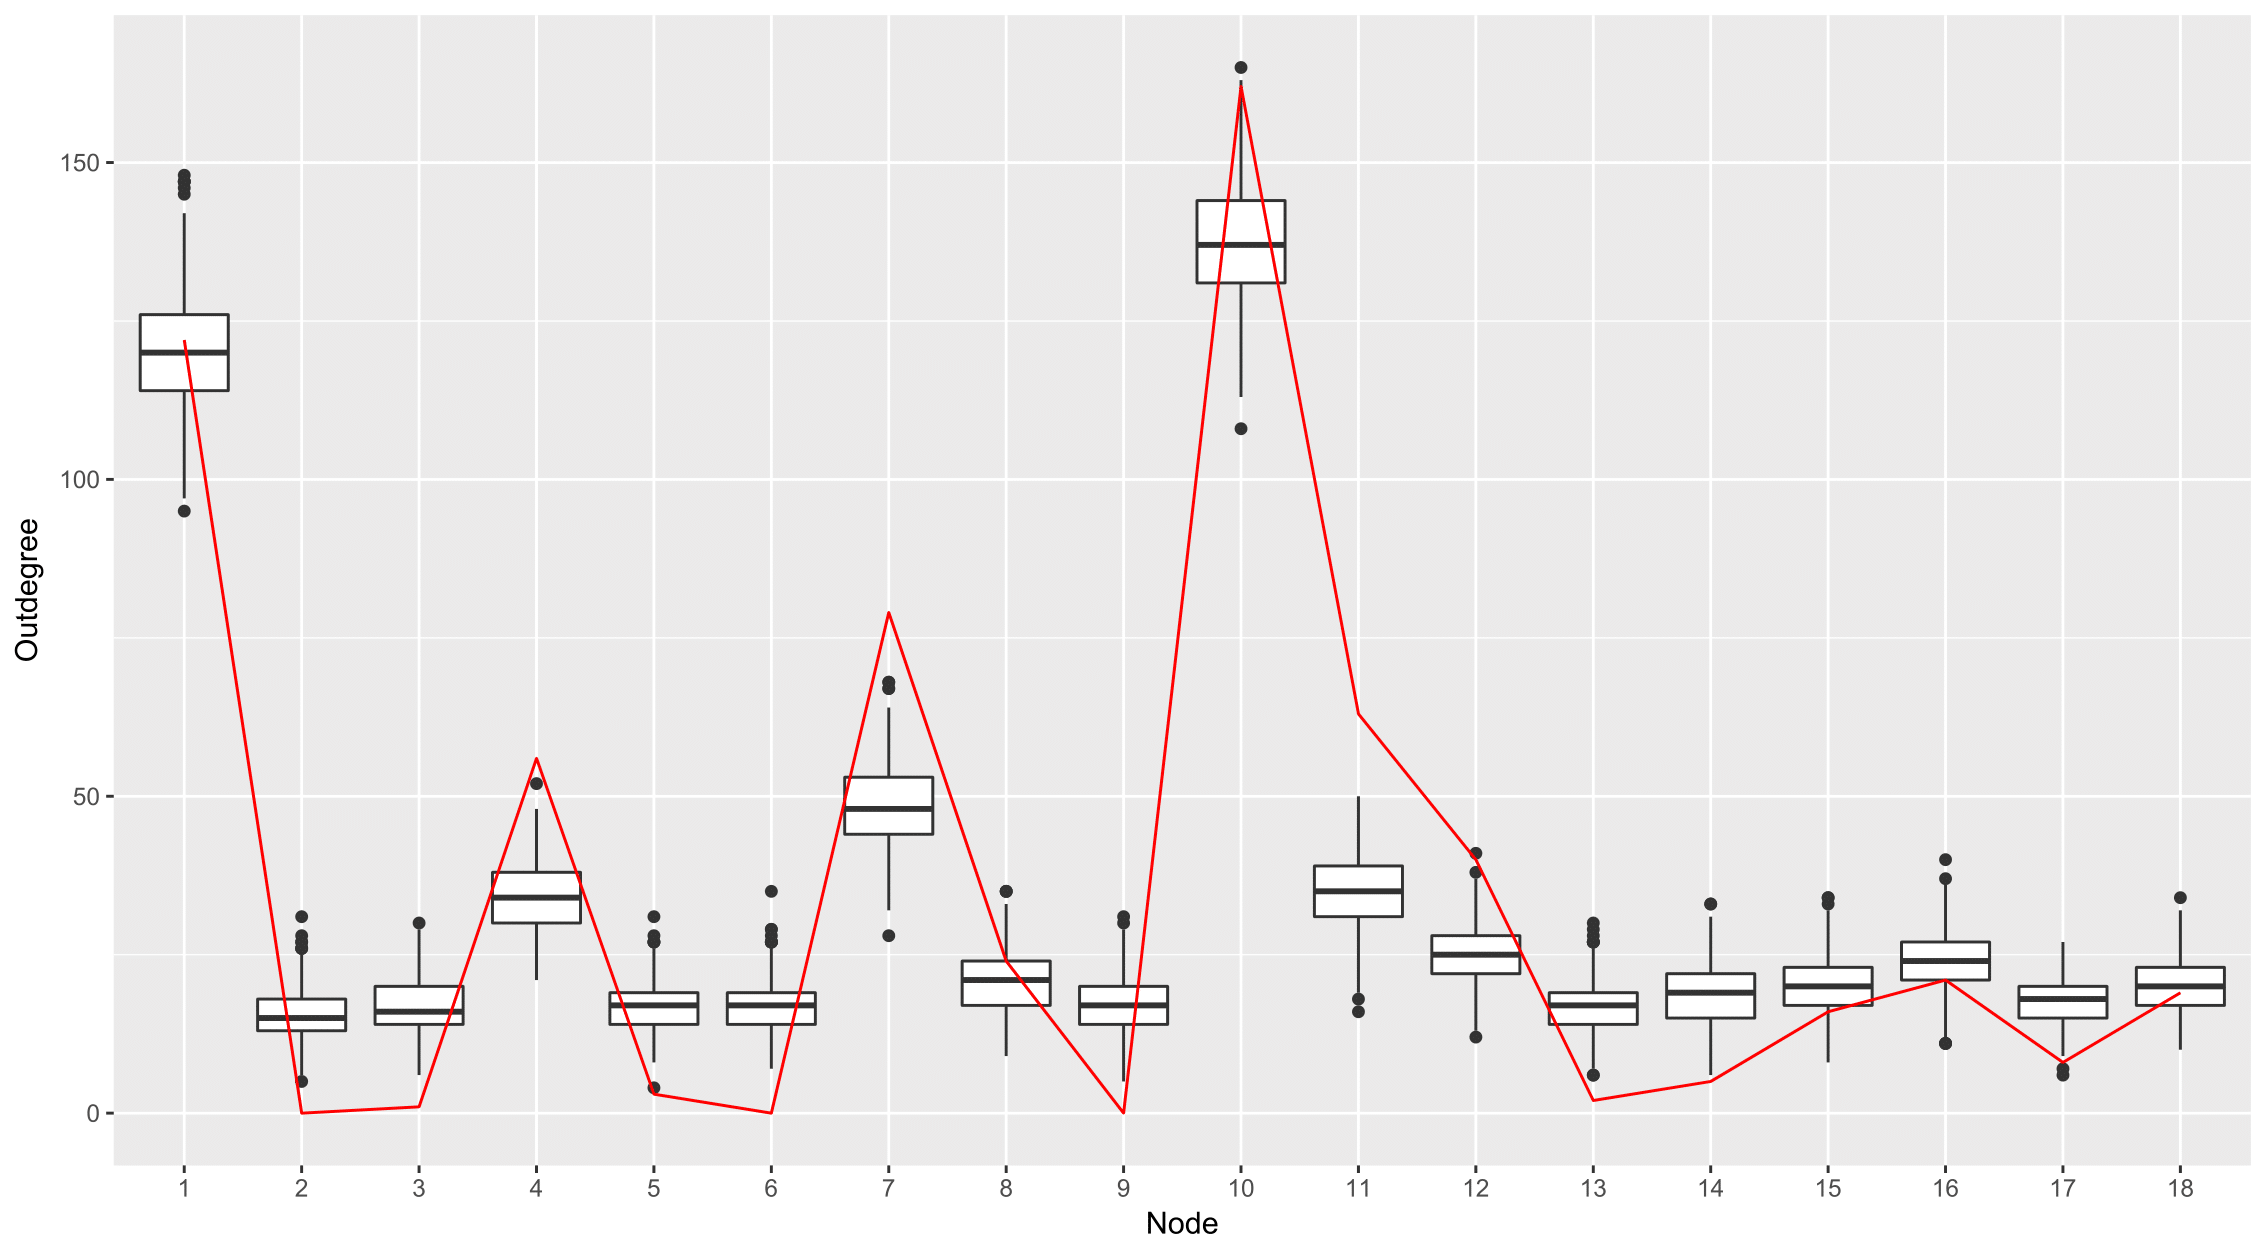
\includegraphics[width=0.495\textwidth]{plots_paper/outdegreenew-1.png}	
		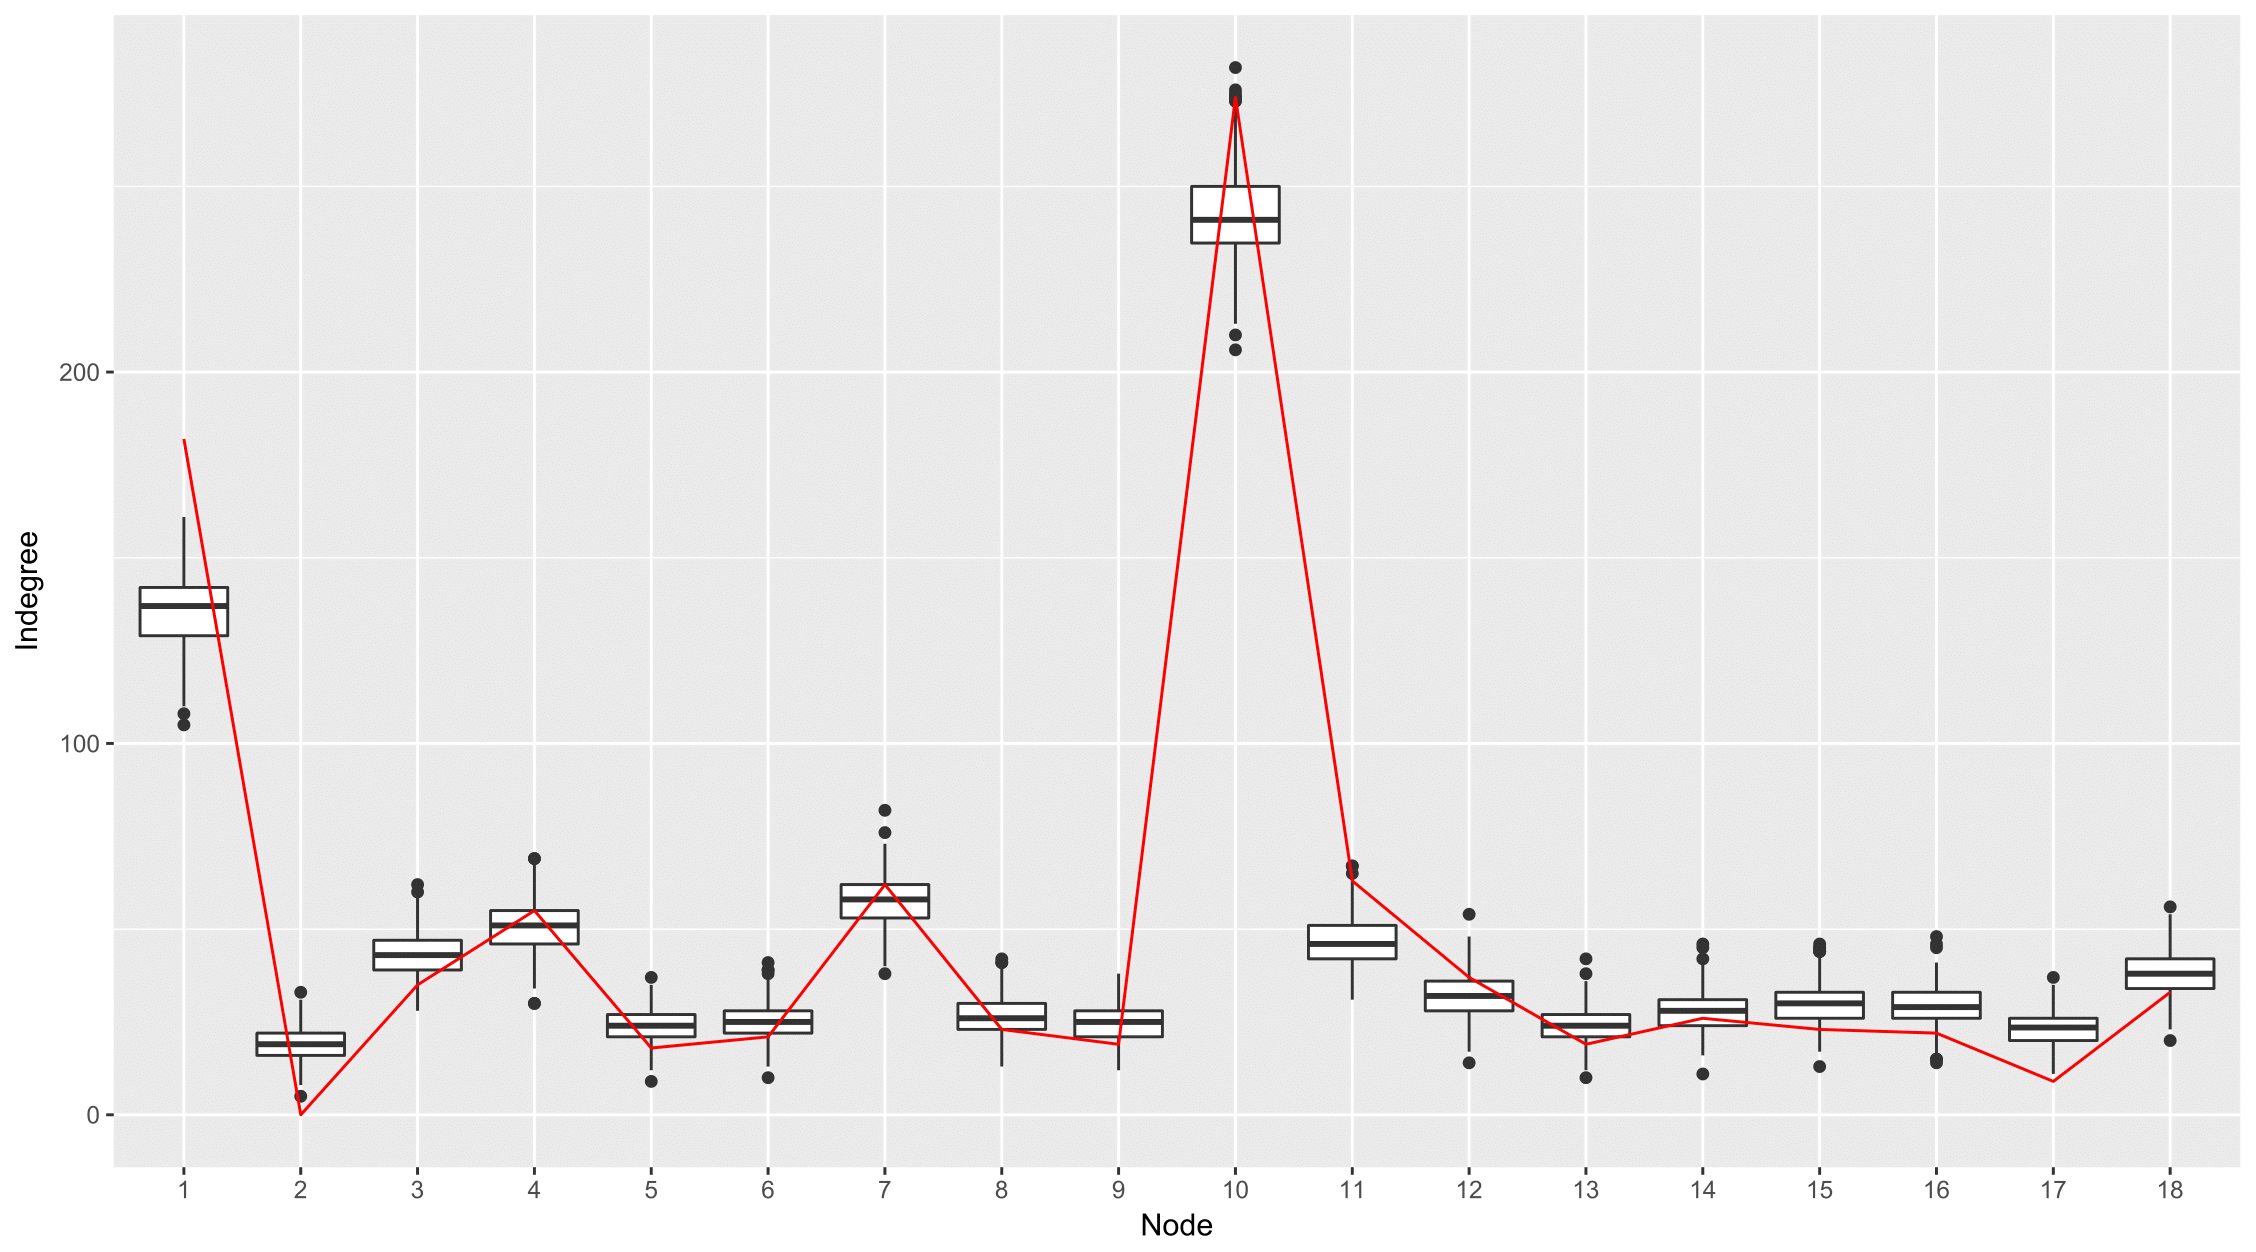
\includegraphics[width=0.495\textwidth]{plots_paper/indegreenew-1.png}	
		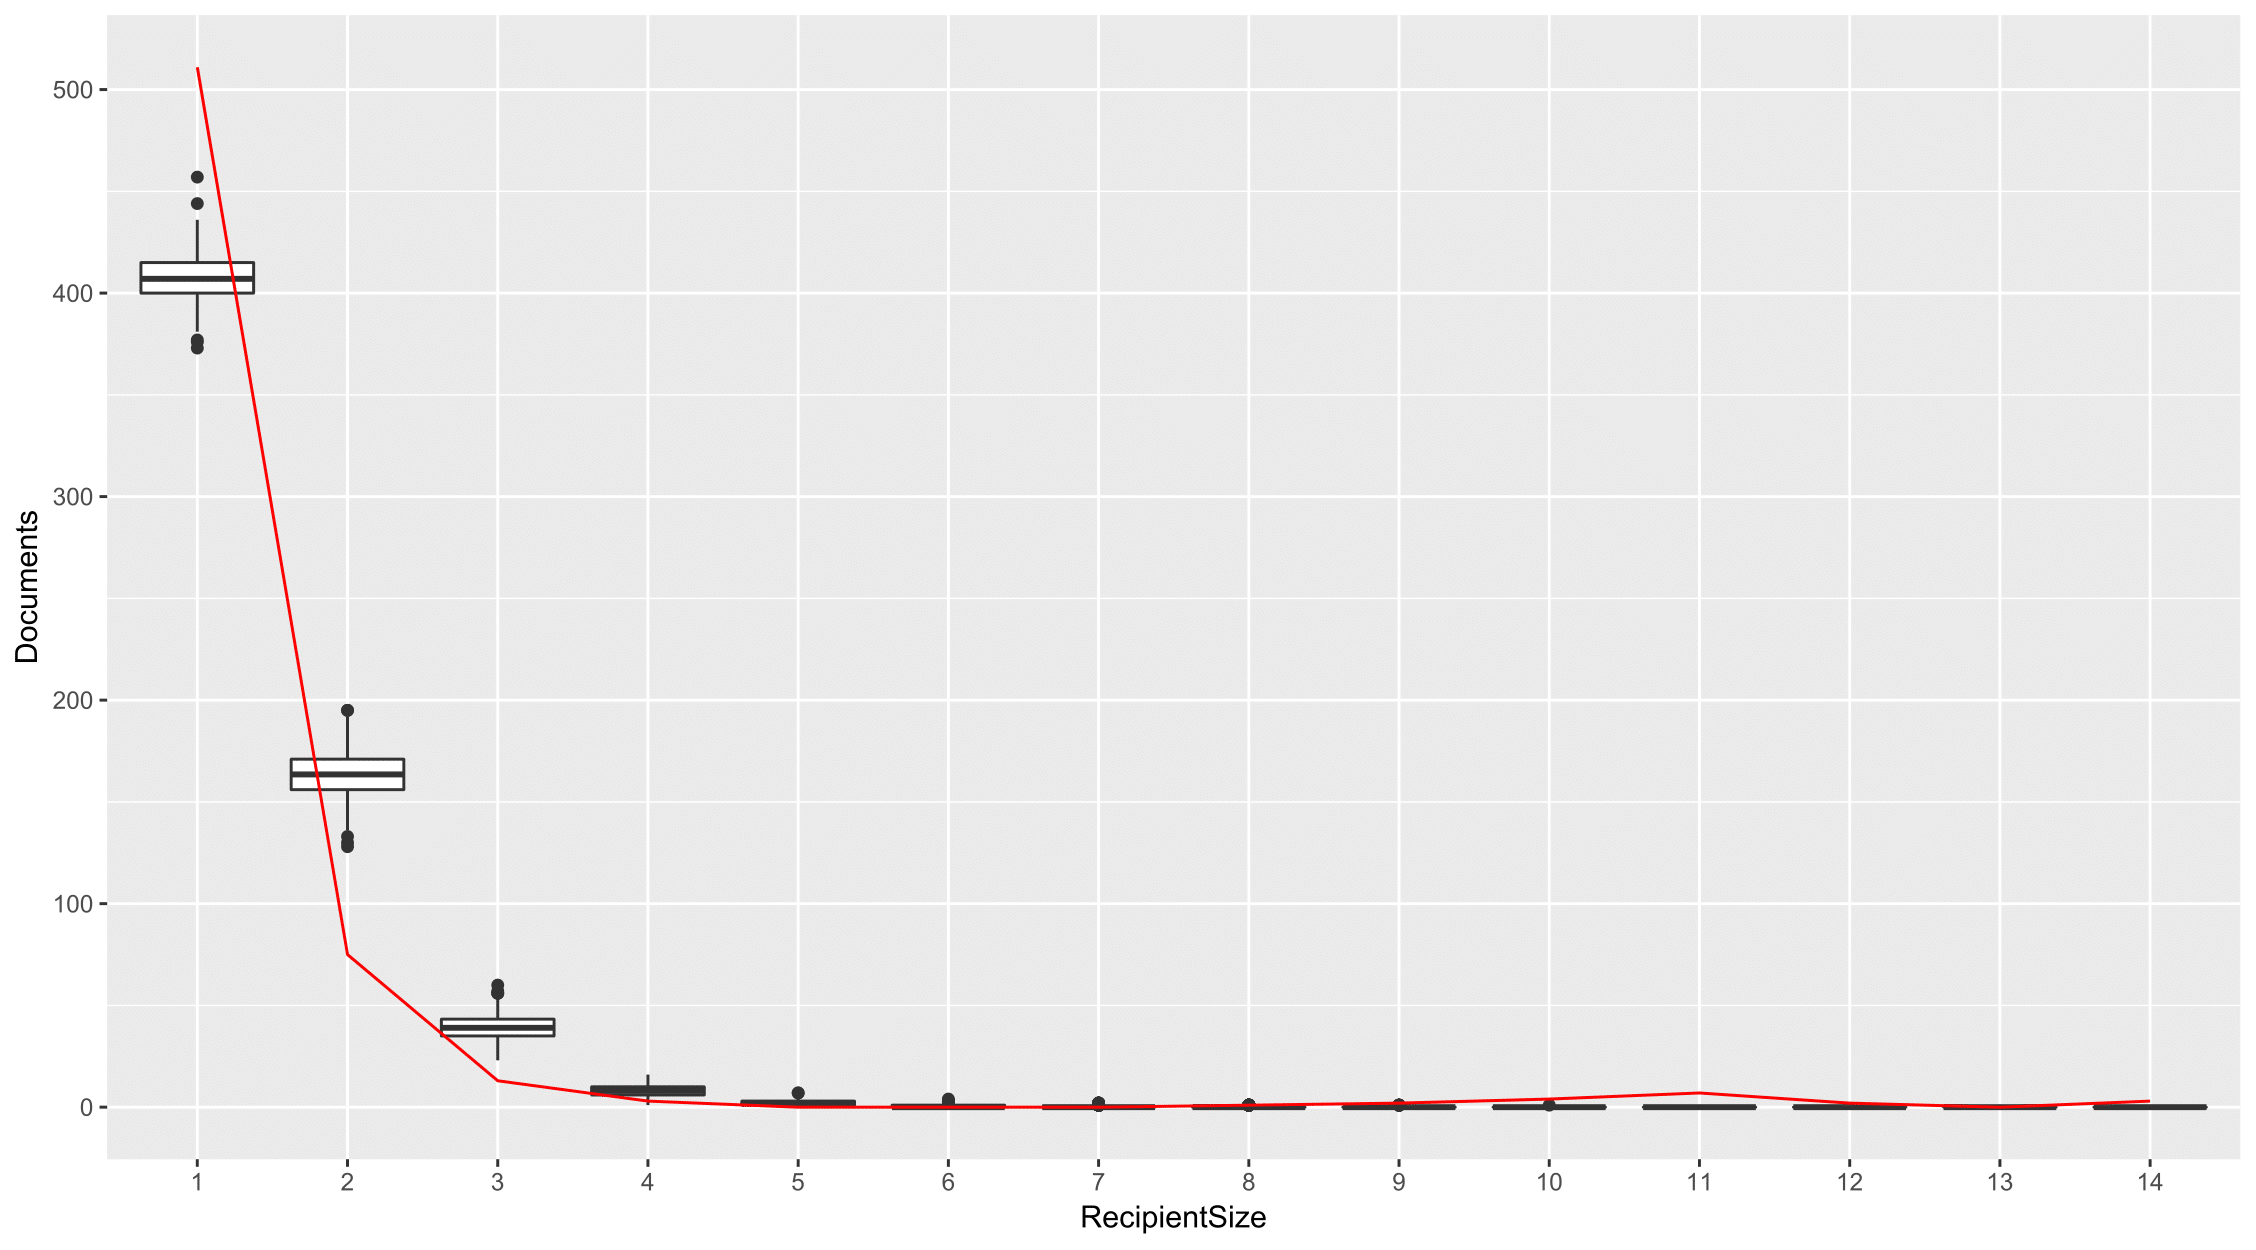
\includegraphics[width=0.495\textwidth]{plots_paper/recipientsizenew-1.png}	
		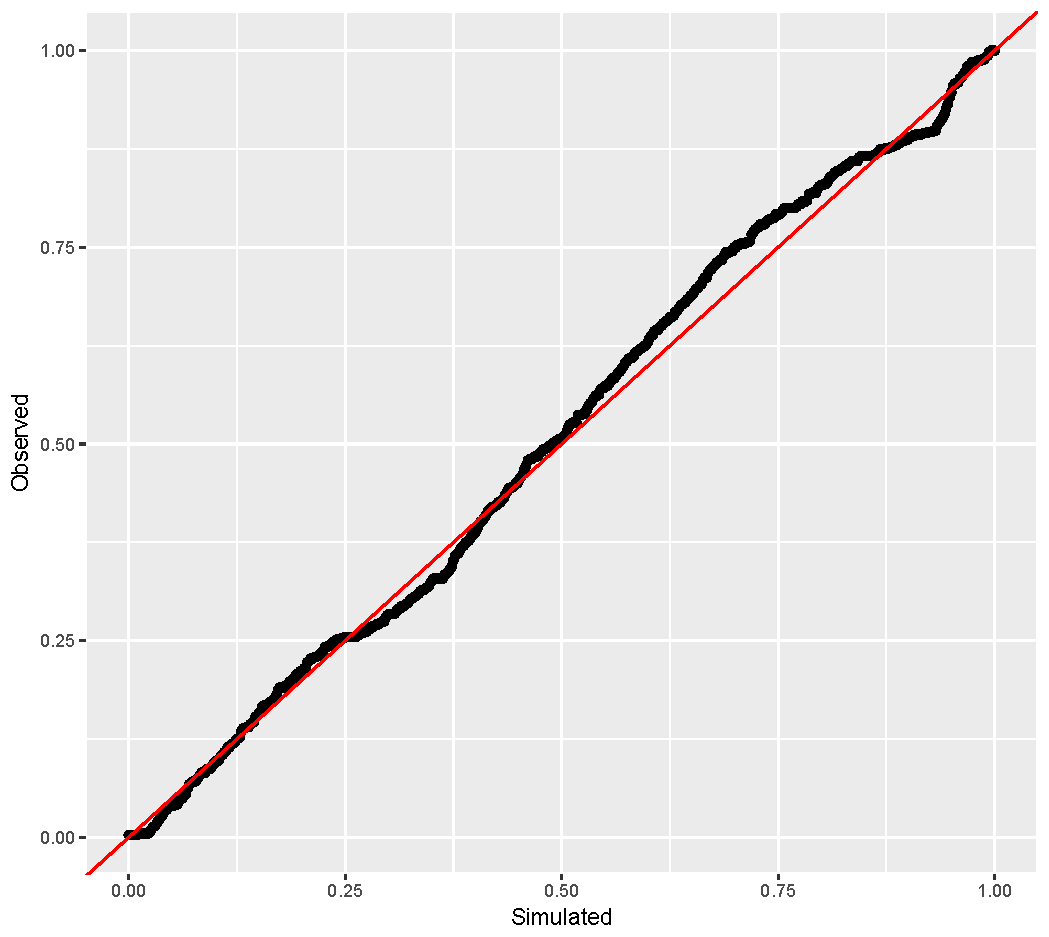
\includegraphics[width=0.31\textwidth]{plots_paper/timeppnew.pdf}
		\caption {PPC results from lognormal distribution: outdegree distribution (\textit{upper left}), indegree distribution (\textit{upper right}), recipient size distribution (\textit{lower left}), and time-increments probability-probability (PP) plot  (\textit{lower right}). Red lines in the first three plot depict the observed statistics, and the red line in the last plot is the diagonal line connecting $(0, 0)$ and $(1, 1)$.}
		\label{figure:PPCresults}
	\end{figure}
	
	Figure \ref{figure:PPCresults} illustrates the results of poterior predictive checks using lognormal distribution. Upper two plots show node-specific degree distributions, where the left one is the boxplots of 500 posterior predictive outdegree statistic and the right plot is the same one for indegree statistic. For both plots, the x-axis represents the node id's from 1 to 18, and the y-axis represents the number of emails sent or received by the node. When compared with the observed outdegree and indegree statistics (red lines), our model recovers the overall distribution of sending and receiving activities across the nodes. For example, node 1 and 10 show significantly higher level of both sending and receiving activities relative to the rest, and the model-simulated data captures those big jumps, without using node-specific indicators. Outdegree distribution of some low-activity nodes are not precisely recovered, however, indegree distribution looks much better. Since we use more information in the recipient selection process (i.e., network effects) while we only rely on minimum time-increments when choosing the observed sender, these results are expected. Lower left plot is the distribution of recipient sizes, where the x-axis spans over the size of recipients 1 to 14 (which is the maximum size of observed recipients) and the y-axis denotes the number of documents with x-number of recipients. The result shows that our model is underestimating single-receiver documents while overestimating documents with two, three, and four recipients. One explanation behind what we observe is that the model is trying to recover so-called ``broadcast'' emails, which are the documents with $\geq 10$ number of recipients, so that the intercept estimate $b_1$ is slightly moved toward right. To improve the goodness of fit for recipient sizes, we can add more covariates (e.g., sender indicators) or assign strong prior structure on $b_1$. In the end, the plot on the lower right is the PP plot for time-increments, which is a graphical measure commonly used for assessing how closely two data sets agree, by plotting the two cumulative distribution functions against each other. The resulting goodness of fit of the diagonal line gives a measure of the difference between the distribution of simulated time-increments and the observed ones, and our PP plot shows that we have great performance in reproducing the observed time distribution. All our findings in previous section is further revealed in the PPC results from exponential distribution, which are attached in Appendix \ref{sec: PPCexp}.
\subsection{Parameter Estimates and Interpretation}\label{subsec:Result_email}
Based on some preliminary experiments, we choose lognormal distribution to model time-to-next-email in Montgomery county email data, thus we estimate the variance parameter $\sigma_\tau^2$ with the prior specified as inverse-Gamma($2, 1$). In this section, we present the results based on 55,000 MCMC outer iterations with a burn-in of 15,000, where we thin by keeping every 40th sample. While the inner iterations for $\boldsymbol{\eta}$ and $\sigma_\tau^2$ are fixed as 1, we use 10 inner iterations for $\boldsymbol{b}$ to adjust for its slower convergence rate.
	\begin{figure}[!b]
	\centering
	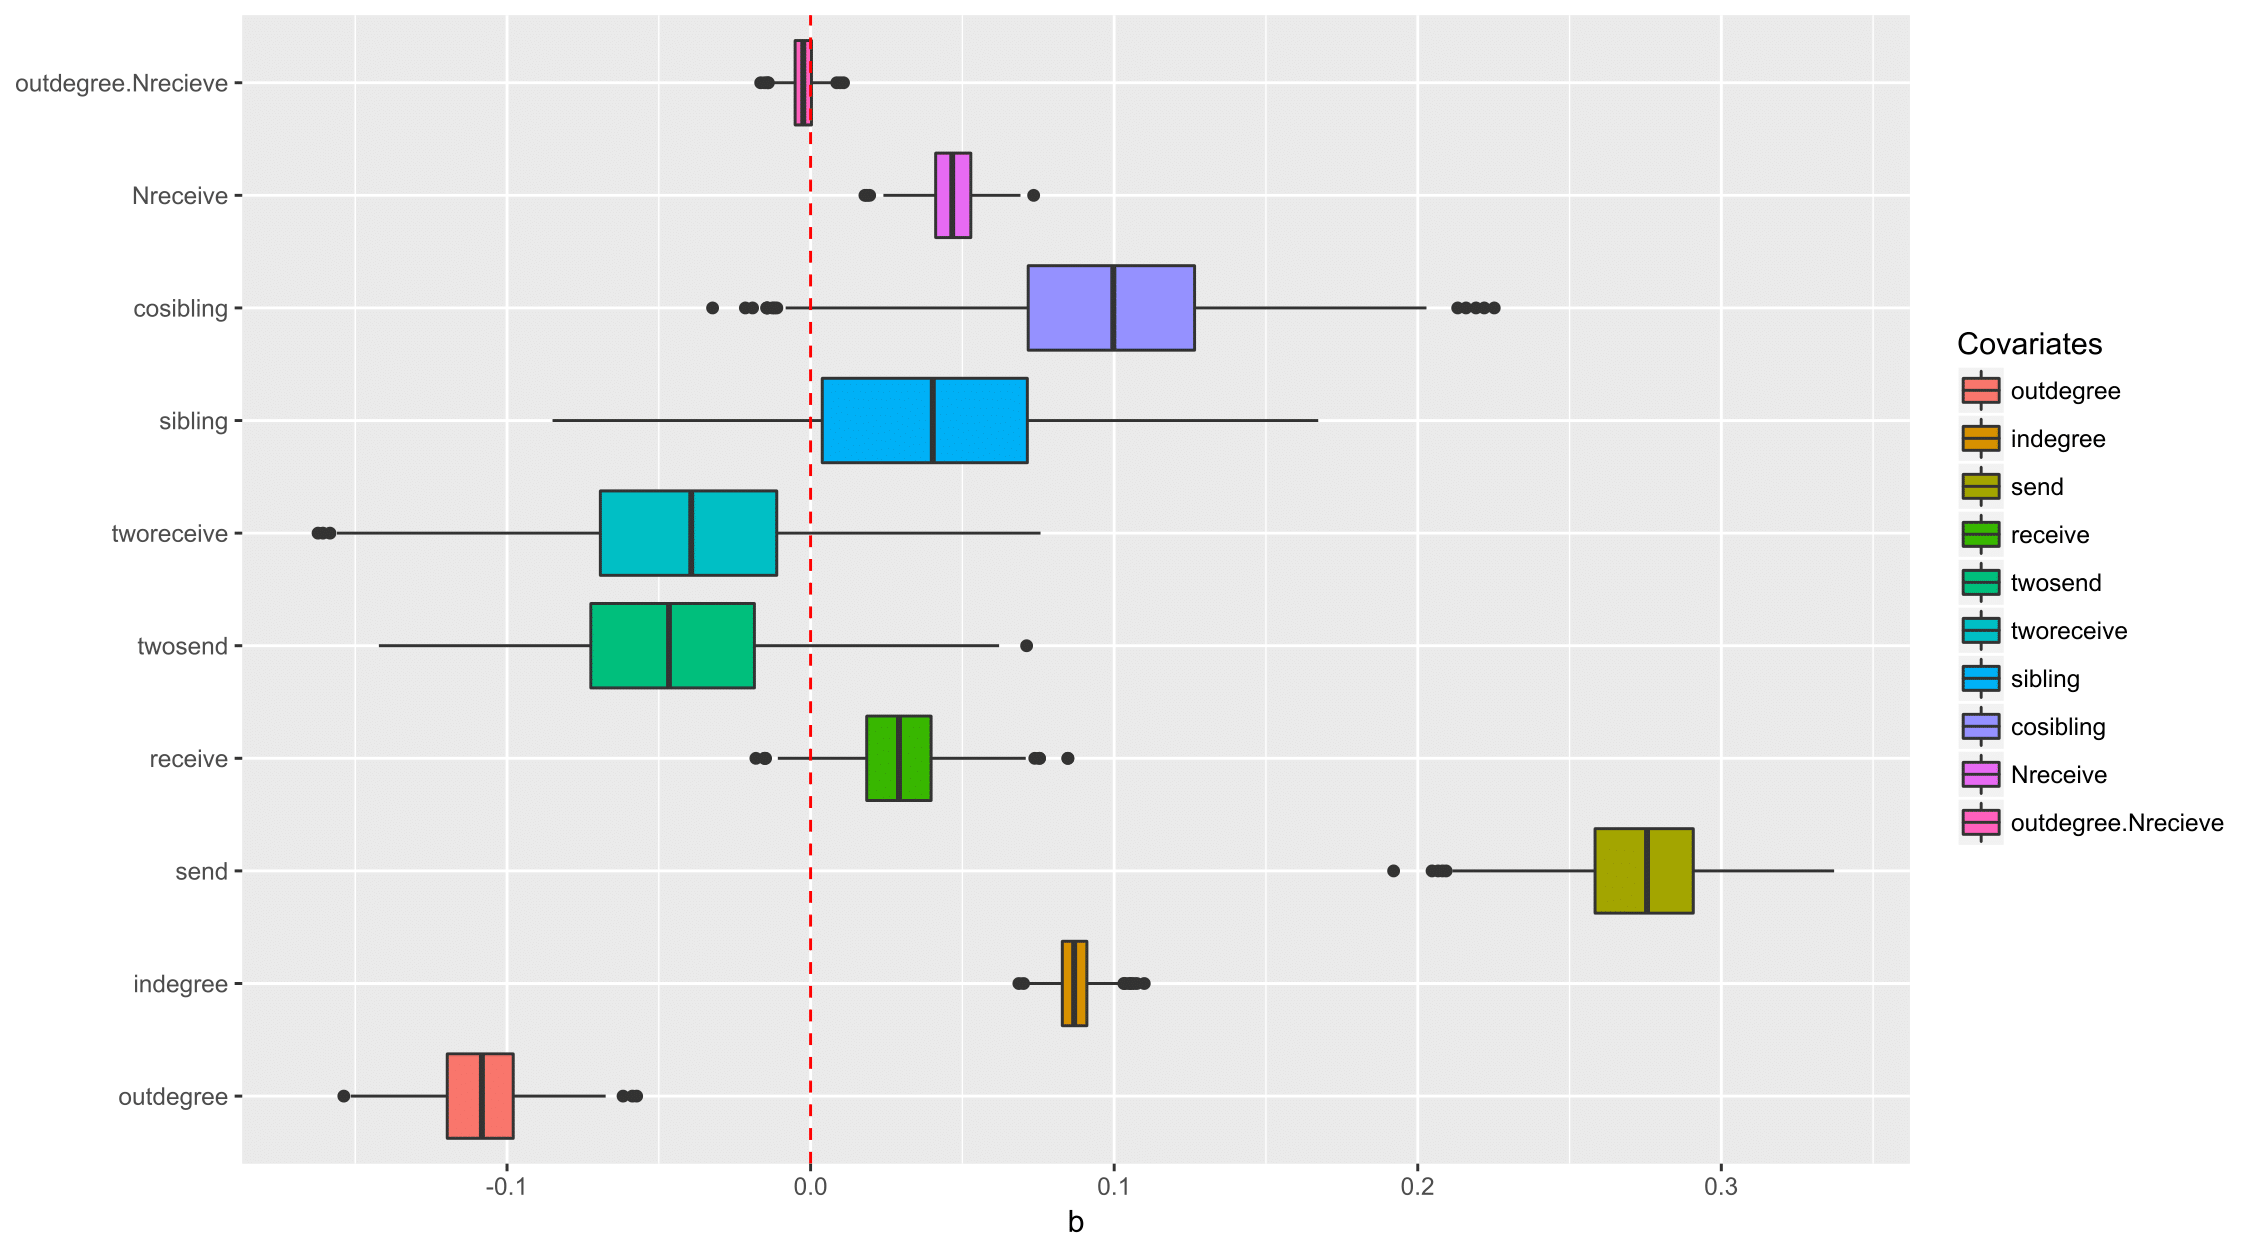
\includegraphics[width=1\textwidth]{plots_paper/best-1.png}	
	\caption {Posterior distribution of $\boldsymbol{b}$ estimates.}
	\label{figure:betaresults}
\end{figure}
	
Figure \ref{figure:betaresults} shows the boxplots summarizing posterior samples of $\boldsymbol{b}$. Since we use logit probability of $\lambda_{adr}$ for edge generating process (Section \ref{subsec: Tie}), we have
\begin{equation*}
\mbox{logit}(\lambda_{adr})=\log\Big(\frac{\lambda_{adr}}{1-\lambda_{adr}}\Big) =b_{1}+b_{2} x_{adr2}\ldots+b_{11}x_{adr11},
\end{equation*}
and can interpret the parameter estimates in terms of odds ratio $\frac{\lambda_{adr}}{1-\lambda_{adr}}=\exp(b_{1}+b_{2} x_{adr2}\ldots+b_{11}x_{adr11})$.
Firstly, we can see that the effect of send (i.e., ``number of times the actor $a$ sent emails to the actor $r$ over the last week'') is positive, implying that if the actor $a$ sent $n$ number of emails to $r$ last week, then the actor $a$ is approximately $\exp(0.274\times n)\approx(1.315)^n$ times more likely to send an email to $r$. Similar interpretation can be applied for the statistics indegree and Nrecieve. For example, as the actor $r$ received $n$ emails and the actor $a$ sent emails to $n$ rececievers over the last week, the actor $a$ is $\exp(0.086\times n)\approx(1.091)^n $ times and $\exp(0.047\times n)\approx(1.048)^n$ times, respectively, more likely to send an email to $r$. On the other hand, outdegree statistic has negative effect---i.e., if the actor $a$ sent $n$ number of emails to anyone last week, then the actor $a$ is approximately $\exp(-0.109\times n)\approx(0.897)^n$ times likely to send an email to $r$---possibly due to its multicollinearity with the statistics send and Nreceive. This can be interpreted as ``if the actor $a$ sent large number of emails over the last week but 1) not to $r$ (excluding the effect of send) or 2) no broadcast or multicast emails (excluding the effect of Nreceive)'' then the actor $a$ is less likely to send an email to $r$. Rest of statistics are not statistically significant because their 95\% credible interval do not include 0. Surprisingly, none of the triadic effects seem to have significant effect on the edge generating process.
	\begin{figure}[!b]
		\centering
		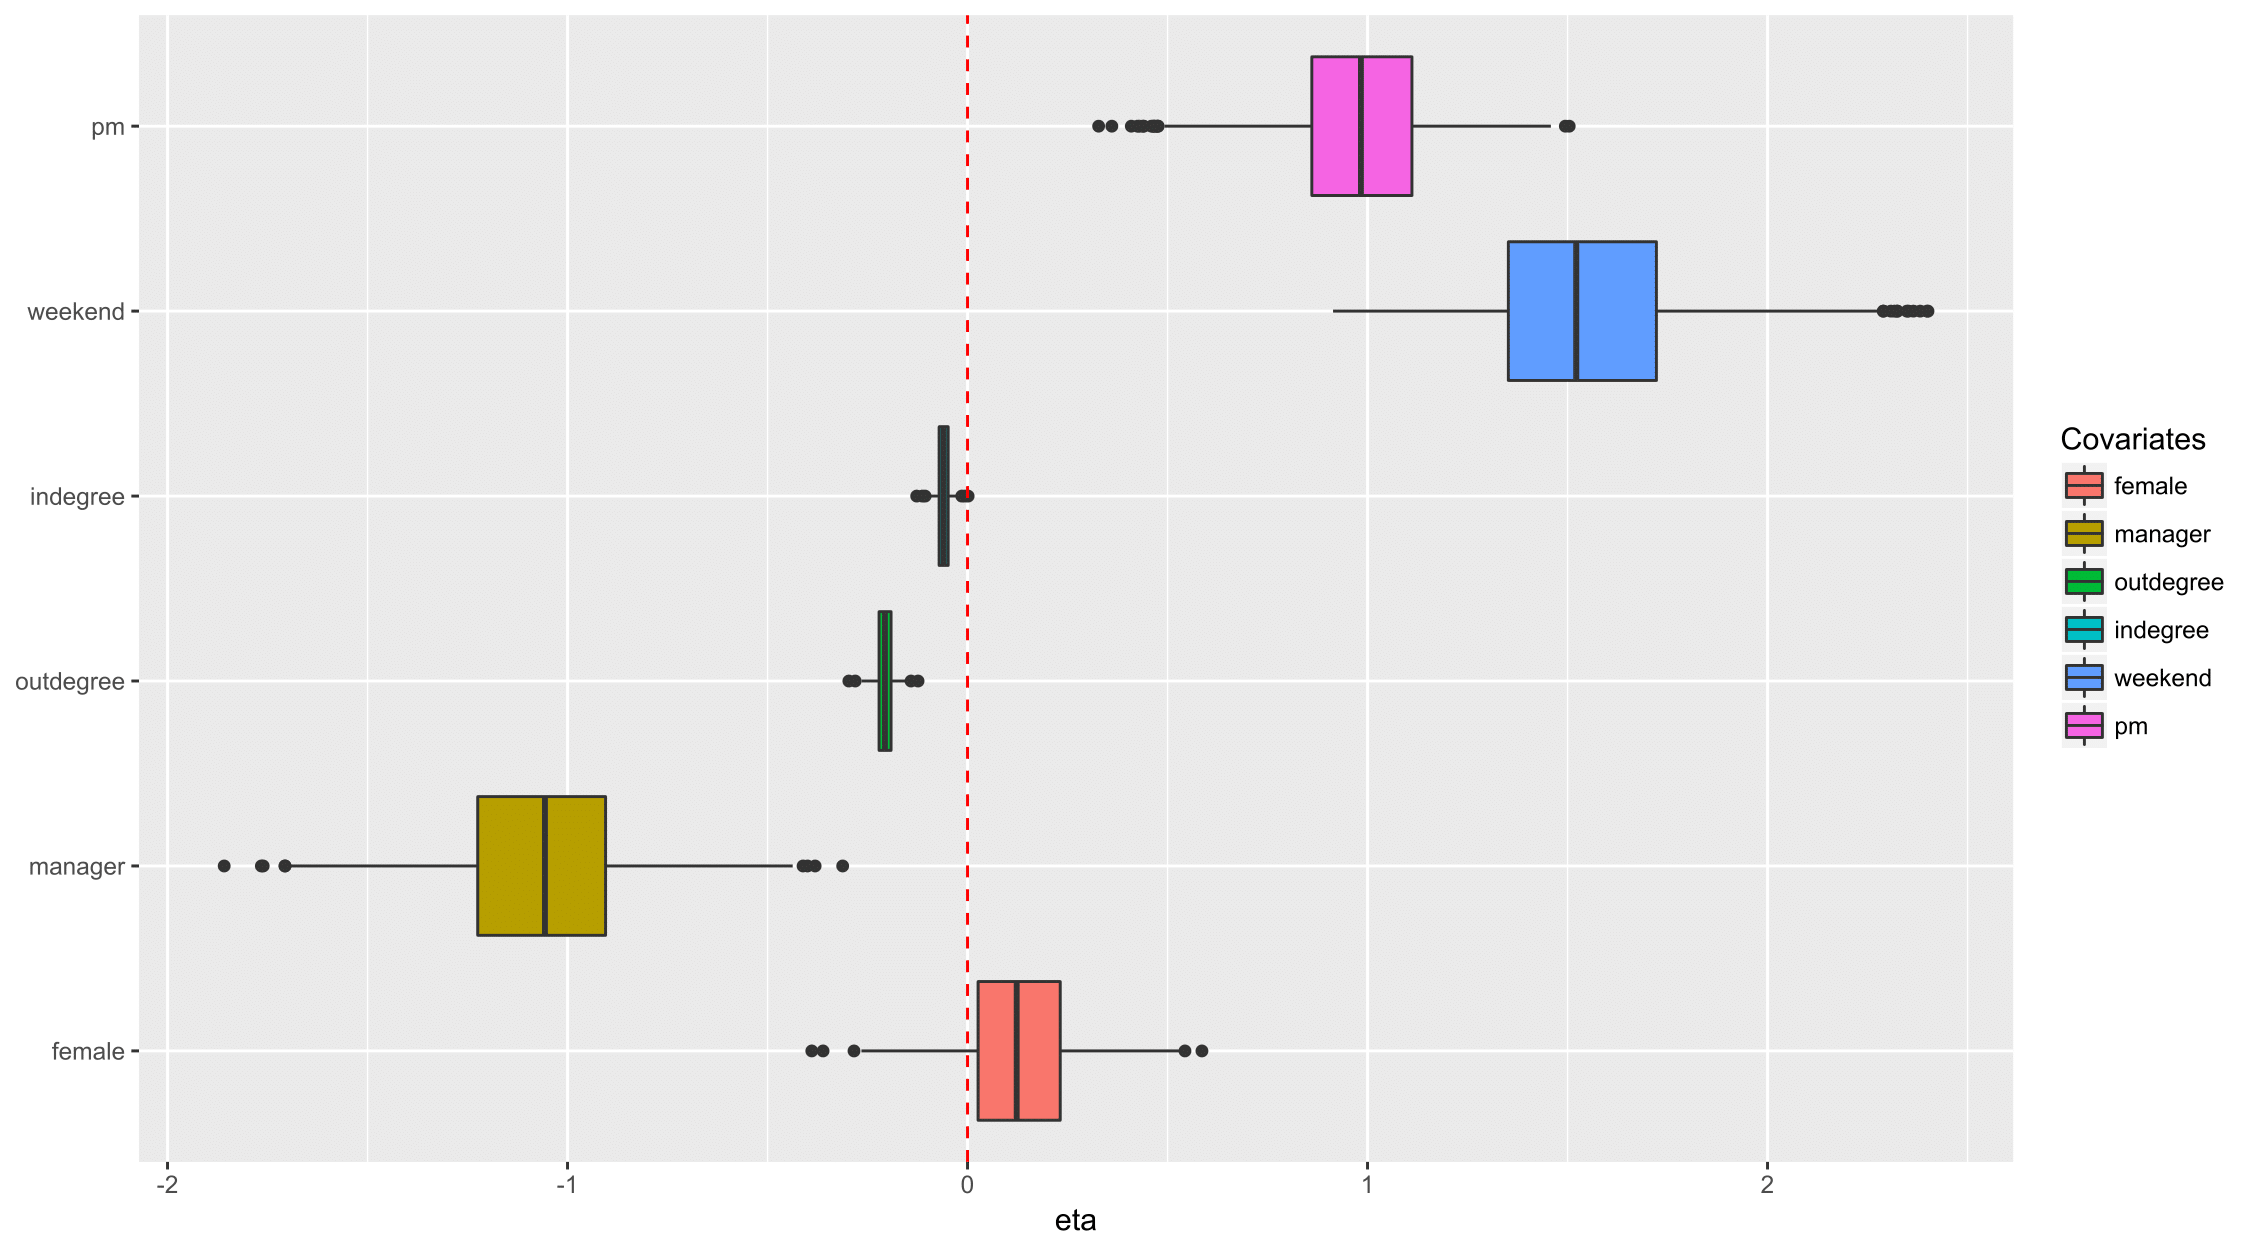
\includegraphics[width=0.89\textwidth]{plots_paper/etaest-1.png}	
		\caption {Posterior distribution of $\boldsymbol{\eta}$ estimates.}
		\label{figure:etaresults}
	\end{figure}
	Figure \ref{figure:etaresults} shows the boxplots summarizing posterior samples of the time-related coefficients $\boldsymbol{\eta}$. For this specific datset, we assume lognormal distribution (Section \ref{subsec:Time}) with the unit of time being an hour, so that the interpretation of $\hat{\boldsymbol{\eta}}$ should be based on
\begin{equation*}
\begin{aligned}
&\log(\tau_{ad}) \sim N(\mu_{ad}, \sigma_\tau^2), \mbox{ with }\\
&\mu_{ad} = \eta_{1}+\eta_{2} y_{ad2}\ldots+\eta_{7}y_{ad7}.
\end{aligned}
\end{equation*}
To begin with, the posterior estimates of two temporal effects---weekend and pm---indicate that if the ${(d-1)}^{th}$ email was sent during the weekend or after 12pm, then the time to $d^{th}$ email is expected to take $\exp(1.552)\approx 4.722$ hours and $\exp(0.980)\approx2.665$ hours longer, respectively, compared to their counterparts (i.e., weekdays and am). On the contrary, the statistics manager, outdegree, and indegree turn out to shorten the time to next email. For example, being a county manager (i.e., the manager of the managers) lowers the expected $\log(\tau_{ad})$ by -1.070, since he or she needs to respond fastly to emails with important decisions. In addition, the manager in general sends or receives a lot more emails which may shorten the response time. This argument is supported by the posterior estimates for outdegree and indegree, where the estimated coefficients are approximately -0.206 and -0.060, respectively. Gender of the department manager is shown to have no significant effect on time-to-next-email. The posterior mean estimate of the variance parameter $\sigma^2_\tau$ is 14.093 with its 95\% credible interval $(12.709, 15.555)$, indicating that there exists huge variability in the time-increments in this data.


\iffalse
\subsection{Case Study 2: International Sanctions}\label{subsec:International Sanctions}
\subsubsection{Threat and Imposition of Sanctions (TIES) Data}\label{subsubsec:TIES}
We processed the threat and imposition of sanctions (TIES) data \citep{morgan2014threat} that includes the records of international sanctions---defined as actions that one or more countries take to limit or end their economic relations with a target country in an effort to persuade that country to change one or more of its policies---from 1945 to 2005.
\subsubsection{Covariates}\label{subsec:Covariates_sanction}
\subsubsection{Parameter Estimation and Interpretation}\label{subsubsec:Result_sanction}
	\subsubsection{Posterior Predictive Checks}\label{subsubsec:PPC_sanction} 	 
		\subsubsection{Prediction Experiment}\label{subsubsec:Experiment_sanction} 
		\fi 
\section{Conclusion}\label{sec:conclusion}
Motivated by the relational event model \citep{Butts2008} and its variants for time-stamped networks, the hyperedge event model (HEM) can effectively learn the underlying edge generating and timestamp generating structures of event data, while allowing flexibity in the covariate specifications and the distributional assumption of time-increments.
Accounting for the hyperedges, we make better use of events with hyperedges than modeling them as duplicate edges. In modeling the timestamps of the events, our generalized linear model (GLM) based formulation eliminates the need to stick with one distribution (e.g., exponential distribution), and we also provide an algorithm for predictive experiment that helps to learn which distribution better fits the data. To sum, the HEM's flexible generative process thus leads to more accurate and precise inference on model parameters.

We have demonstrated effectiveness of our model by analyzing Montgomery County government emails, which includes numerous hyperedges. The estimated covariate effects reveal that the HEM is able to understand the structural dynamics similar to those used in the exponential random graph model (ERGM), while the model additionally allows separate covariates and the corresponding parameters for edge and timestamp generating processes. Although we illustrate the entire framework and application in the context
of one type of hyperedges, a single sender and multiple recipients, our model can be easily extended to allow the opposite case, a single recipient and multiple senders, by slight modification of the generating process. This extension involves promissing applications including international sanctions and co-sponsorship of bills. Furthermore, while currently the model's applicability is limited to small-sized networks since we assume fixed set of nodes across entire timepoints, we can adjust the model to allow time-varying nodes or improve its computational efficiency such that the model is well applicable to large-scale networks. Considering the recent explosion of network dataset with huge number of nodes (e.g., online comnunications), the development of model adjustments for better applicability are objects of future work.
\bibliographystyle{agsm}
\bibliography{multicastnetwork}
\begin{appendices}
\section{Normalizing Constant of MB$_{Gibbs}$}\label{sec: non-empty Gibbs measure}
Our probability measure ``MB$_{Gibbs}$''---the multivariate Bernoulli distribution with non-empty Gibbs measure \citep{fellows2017removing}---defines the probability of author $a$ selecting the binary recipient vector $\boldsymbol{u}_{ad}$ as
\begin{equation*} 
\begin{aligned}
& P(\boldsymbol{u}_{ad}|\boldsymbol{\lambda}_{ad} ) = \frac{\exp\Big\{ \mbox{log}\big(\text{I}(\lVert \boldsymbol{u}_{ad} \rVert_1 > 0)\big) + \sum_{r \neq a} \lambda_{adr}u_{adr} \Big\}}{Z(\boldsymbol{\lambda}_{ad})}.
\end{aligned}
\end{equation*}

To use this distribution efficiently, we derive a closed-form expression for $Z(\boldsymbol{\lambda}_{id})$ that does not require brute-force summation over the support of $\boldsymbol{u}_{ad}$ (\textit{i.e.} $\forall \boldsymbol{u}_{ad} \in [0,1]^A$). We recognize that if $\boldsymbol{u}_{ad}$ were drawn via independent Bernoulli distributions in which $P({u}_{adr}=1|\delta, \boldsymbol{\lambda}_{ad})$ was given by logit$(\lambda_{adr})$, then 
\begin{equation*}
P(\boldsymbol{u}_{ad}|\boldsymbol{\lambda}_{ad}) \propto \exp\Big\{\sum_{r \neq a } \lambda_{adr}u_{adr}\Big\}.  	 
\end{equation*}
This is straightforward to verify by looking at 
\begin{equation*}
\begin{aligned}
&P(u_{adr}=1|\boldsymbol{u}_{ad[-r]}, \boldsymbol{\lambda}_{ad})
=\frac{ \exp{(\lambda_{adr})}}{\exp{(\lambda_{adr})} + 1}.\end{aligned}\end{equation*}
We denote the logistic-Bernoulli normalizing constant as $Z^{l}(\boldsymbol{\lambda}_{ad})$, which is defined as 
\begin{equation*}
Z^{l}(\delta,\boldsymbol{\lambda}_{ad})=\sum_{\boldsymbol{u}_{ad} \in [0,1]^{A}} \exp\Big\{\sum_{r\neq a} \lambda_{adr}u_{adr}\Big\}.
\end{equation*}
Now, since 
\begin{equation*}
\begin{aligned}
&\exp\Big\{ \mbox{log}\Big(\text{I}(\lVert \boldsymbol{u}_{ad} \rVert_1 > 0)\Big) + \sum_{r \neq a} \lambda_{adr}u_{adr} \Big\}\\&= \exp\Big\{  \sum_{r \neq a} \lambda_{adr}u_{adr} \Big\},
\end{aligned}
\end{equation*}
except when $\lVert \boldsymbol{u}_{ad} \rVert_1=0$, we note that 
\begin{equation*}
\begin{aligned}
Z(\boldsymbol{\lambda}_{ad})& = Z^{l}(\boldsymbol{\lambda}_{ad}) -\exp\Big\{ \sum\limits_{\forall u_{adr}=0}\lambda_{adr}u_{adr} \Big\}
\\& = Z^{l}(\lambda_{a}^{(d)}) -  1.
\end{aligned}
\end{equation*}
We can therefore derive a closed form expression for $Z(\delta,\boldsymbol{\lambda}_{ad})$ via a closed form expression for $Z^{l}(\delta,\boldsymbol{\lambda}_{ad})$. This can be done by looking at the probability of the zero vector under the logistic-Bernoulli model:
\begin{equation*}
\begin{aligned}
&\frac{\exp\Big\{ \sum\limits_{\forall u_{adr}=0}\lambda_{adr}u_{adr} \Big\}}{Z^{l}(\boldsymbol{\lambda}_{ad})}= \prod_{r \neq a}   \Big(1-\frac{ \exp{(\lambda_{adr})}}{\exp{(\lambda_{adr})} + 1}\Big).
\end{aligned}  
\end{equation*}
Then, we have 
\begin{equation*}
\begin{aligned}
& \frac{1}{Z^{l}(\boldsymbol{\lambda}_{ad})} &= \prod\limits_{r \neq a}\frac{1}{ \exp(\lambda_{adr})+ 1}.
\end{aligned}  
\end{equation*}
Finally, the closed form expression for the normalizing constant is  \begin{equation*}
\begin{aligned}Z(\boldsymbol{\lambda}_{ad}) = \prod_{r \neq a } \big(\mbox{exp}(\lambda_{adr}) + 1\big)-1.
\end{aligned}  
\end{equation*}
 \section{PPC Results from Exponential Distribution}\label{sec: PPCexp}
 	\begin{figure}[H]
 		\centering
 		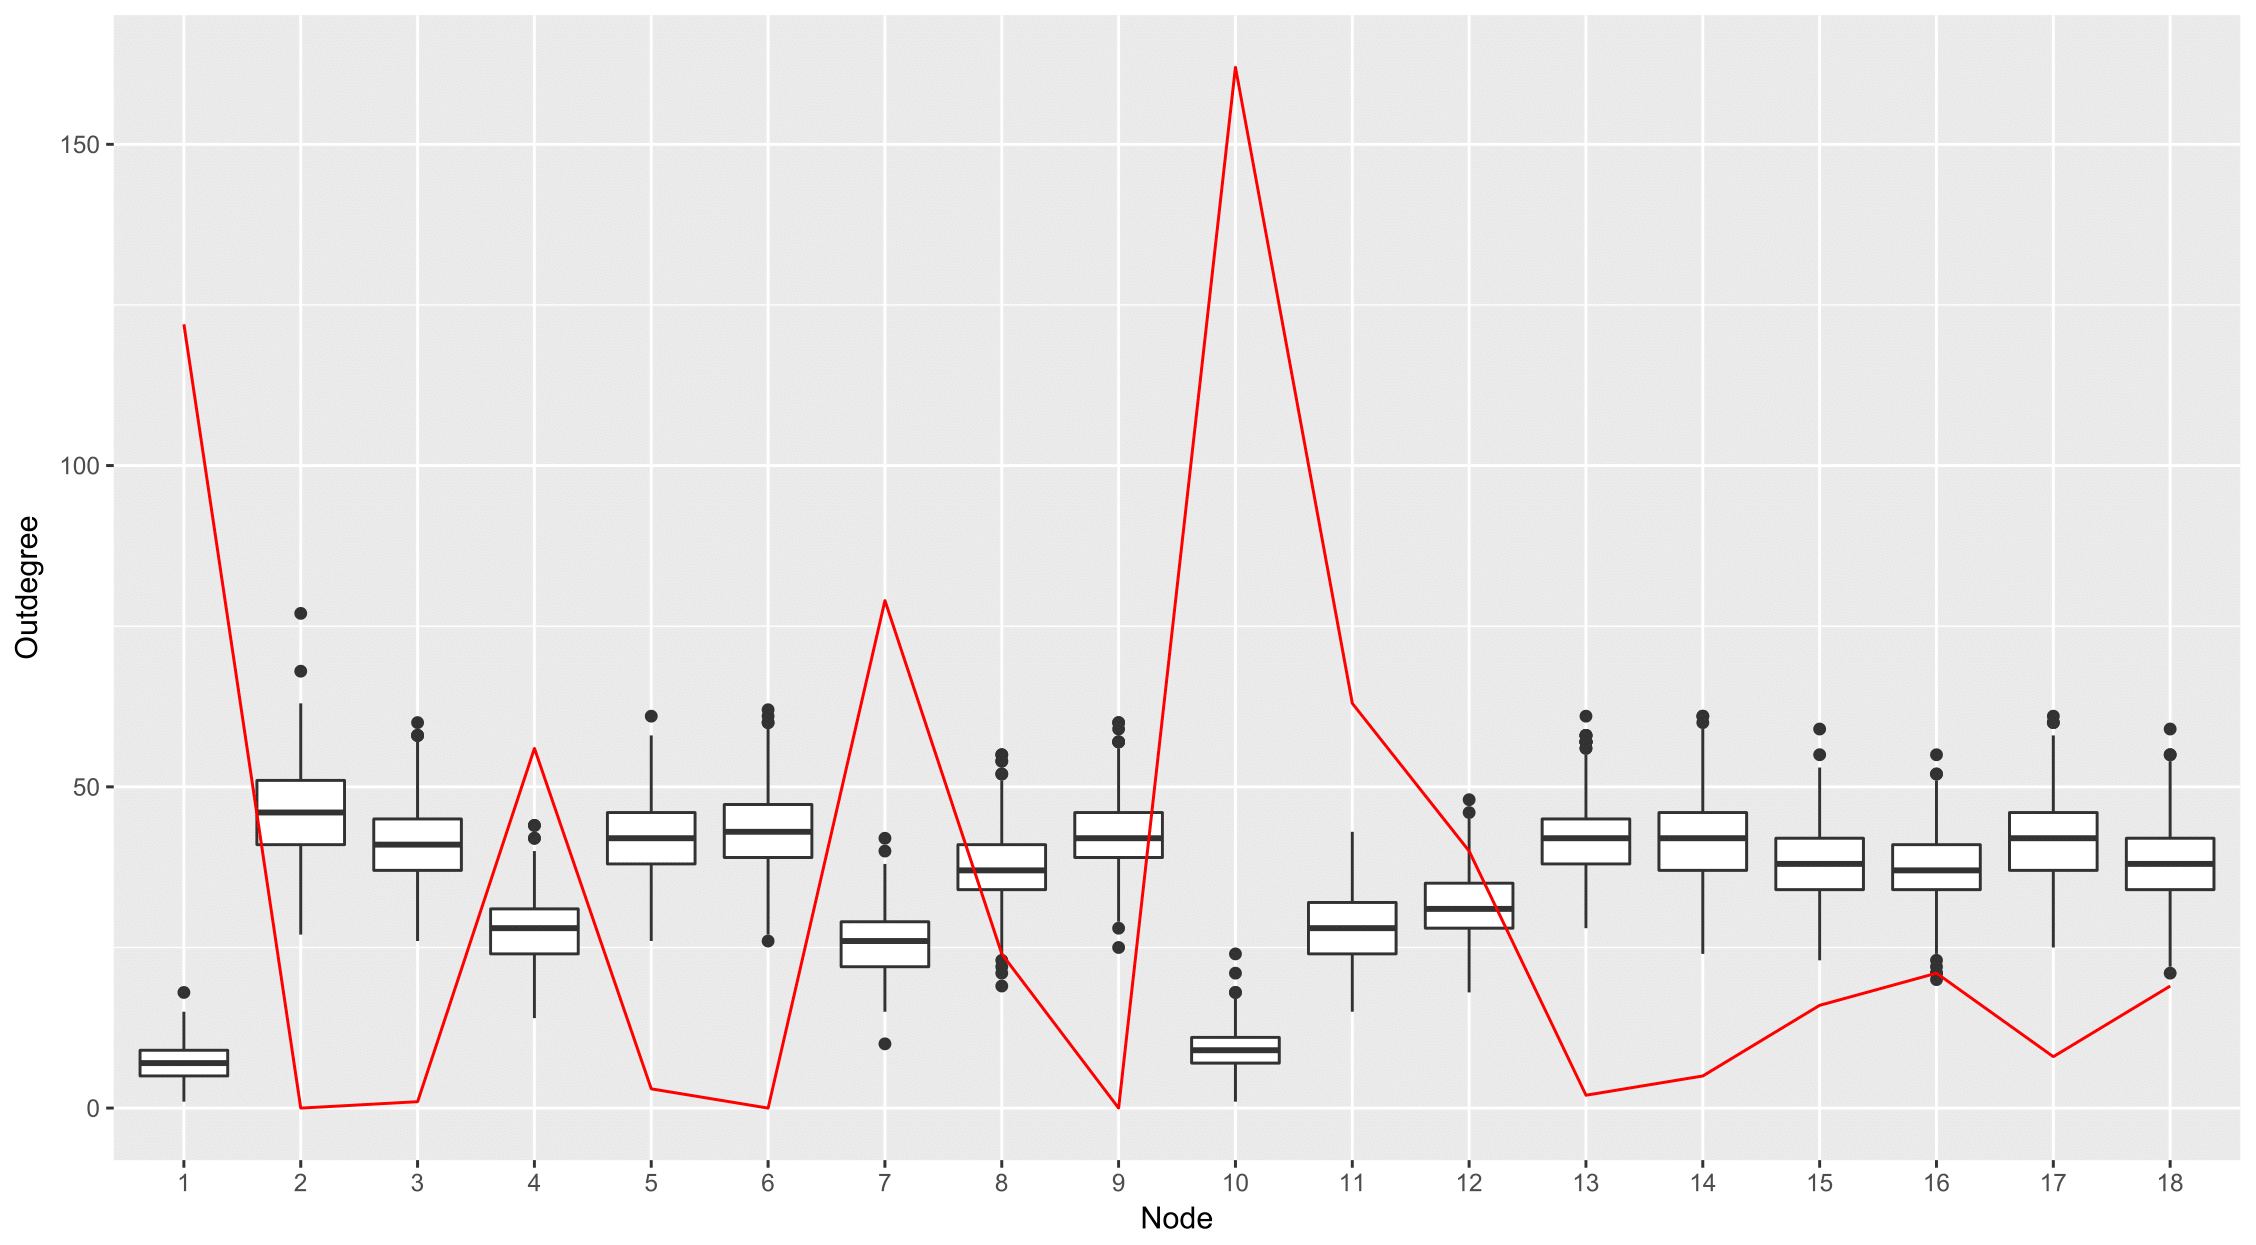
\includegraphics[width=0.495\textwidth]{plots_paper/outdegree_exp-1.png}	
 		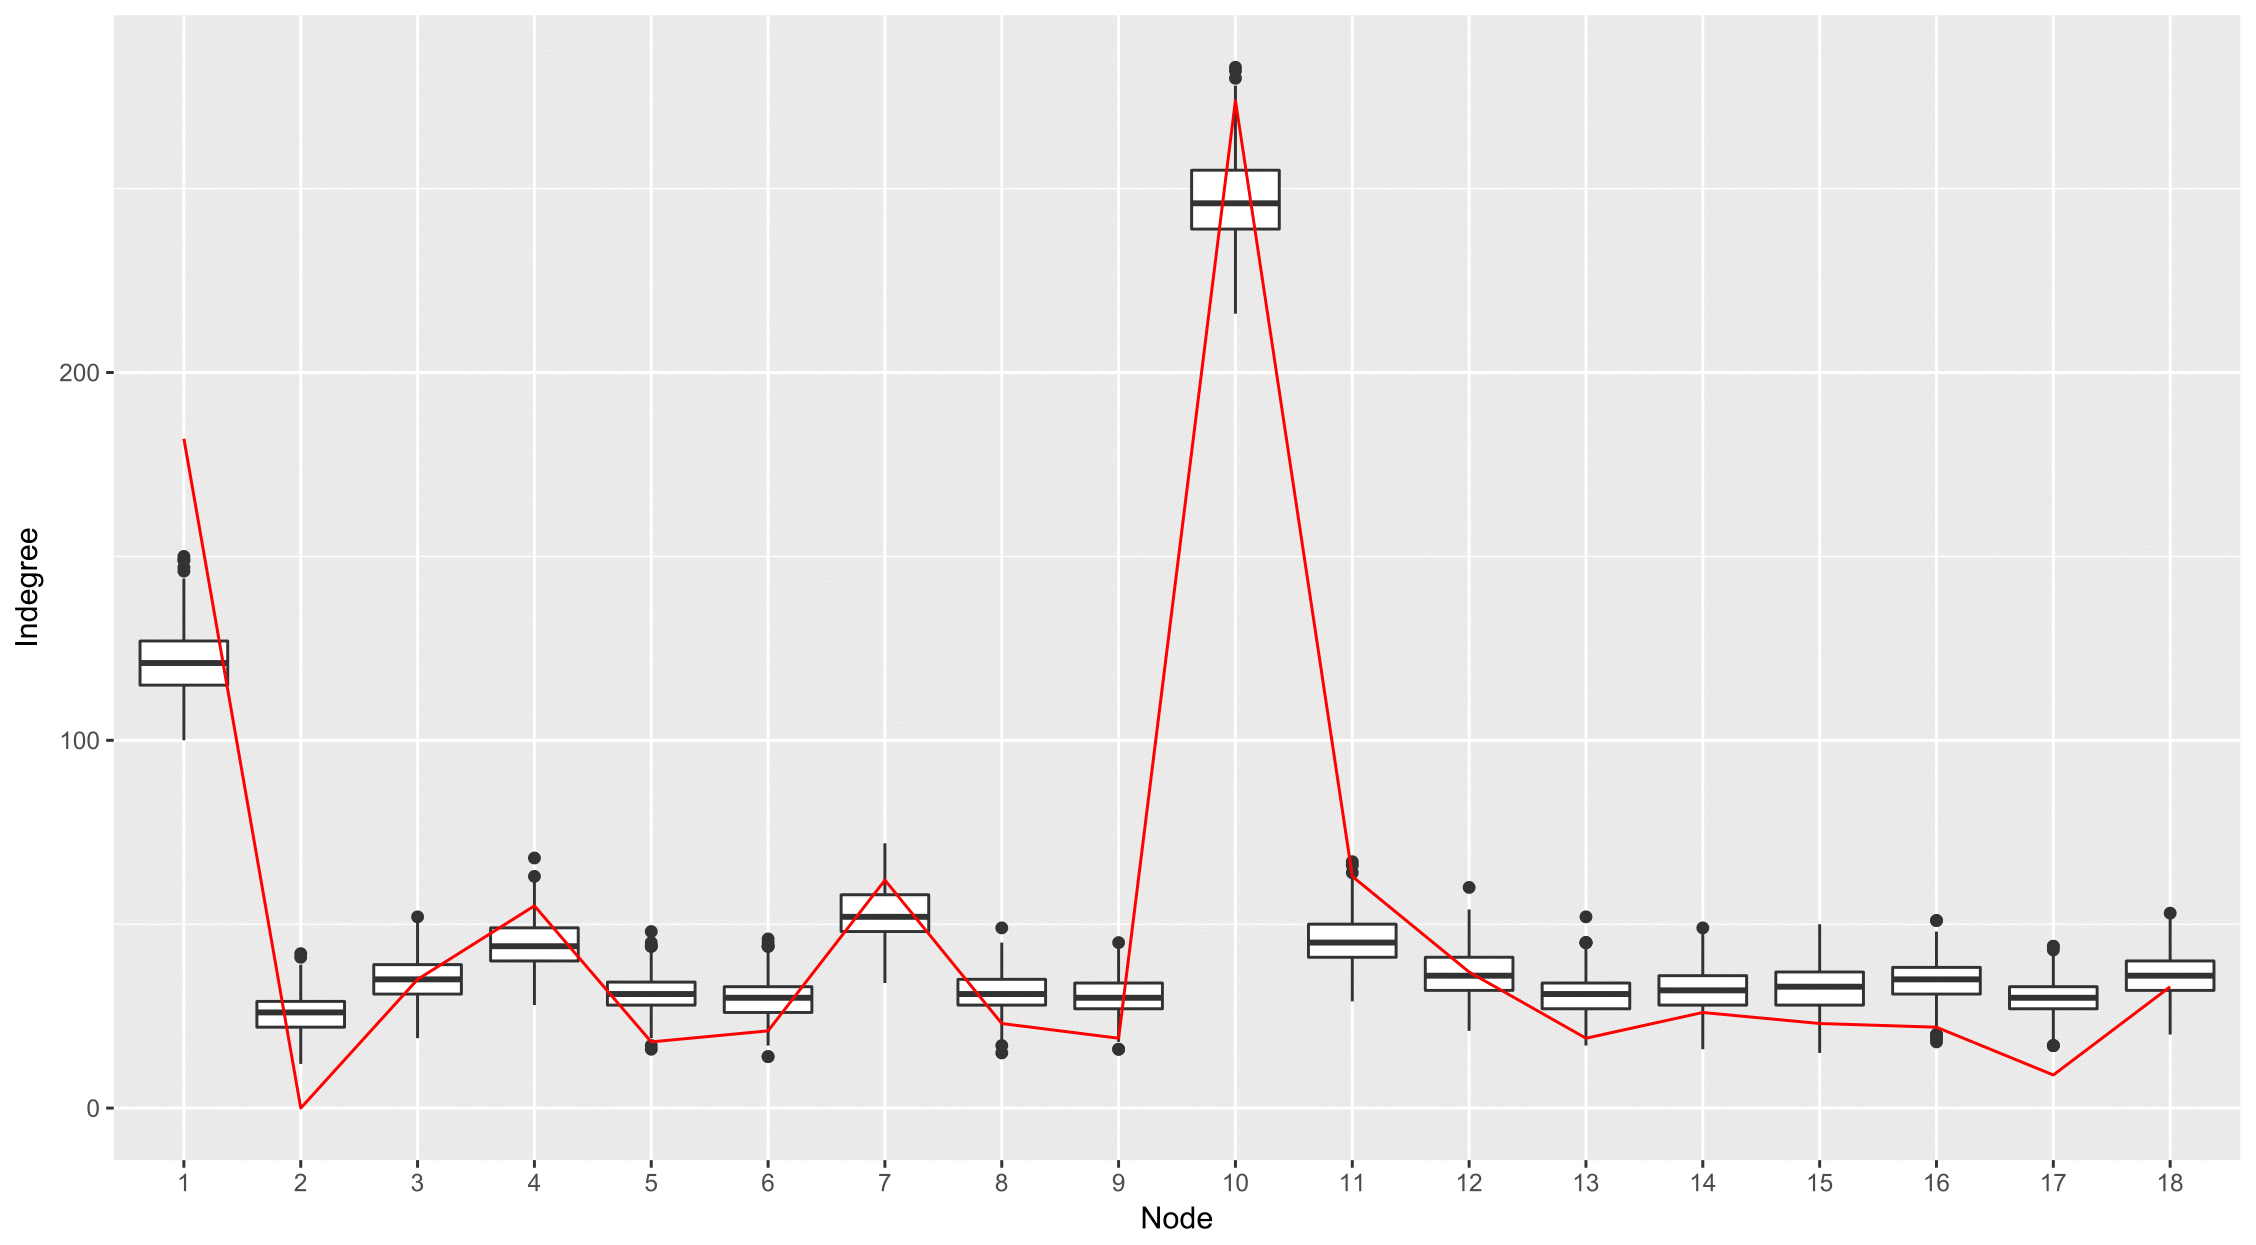
\includegraphics[width=0.495\textwidth]{plots_paper/indegree_exp-1.png}	
 		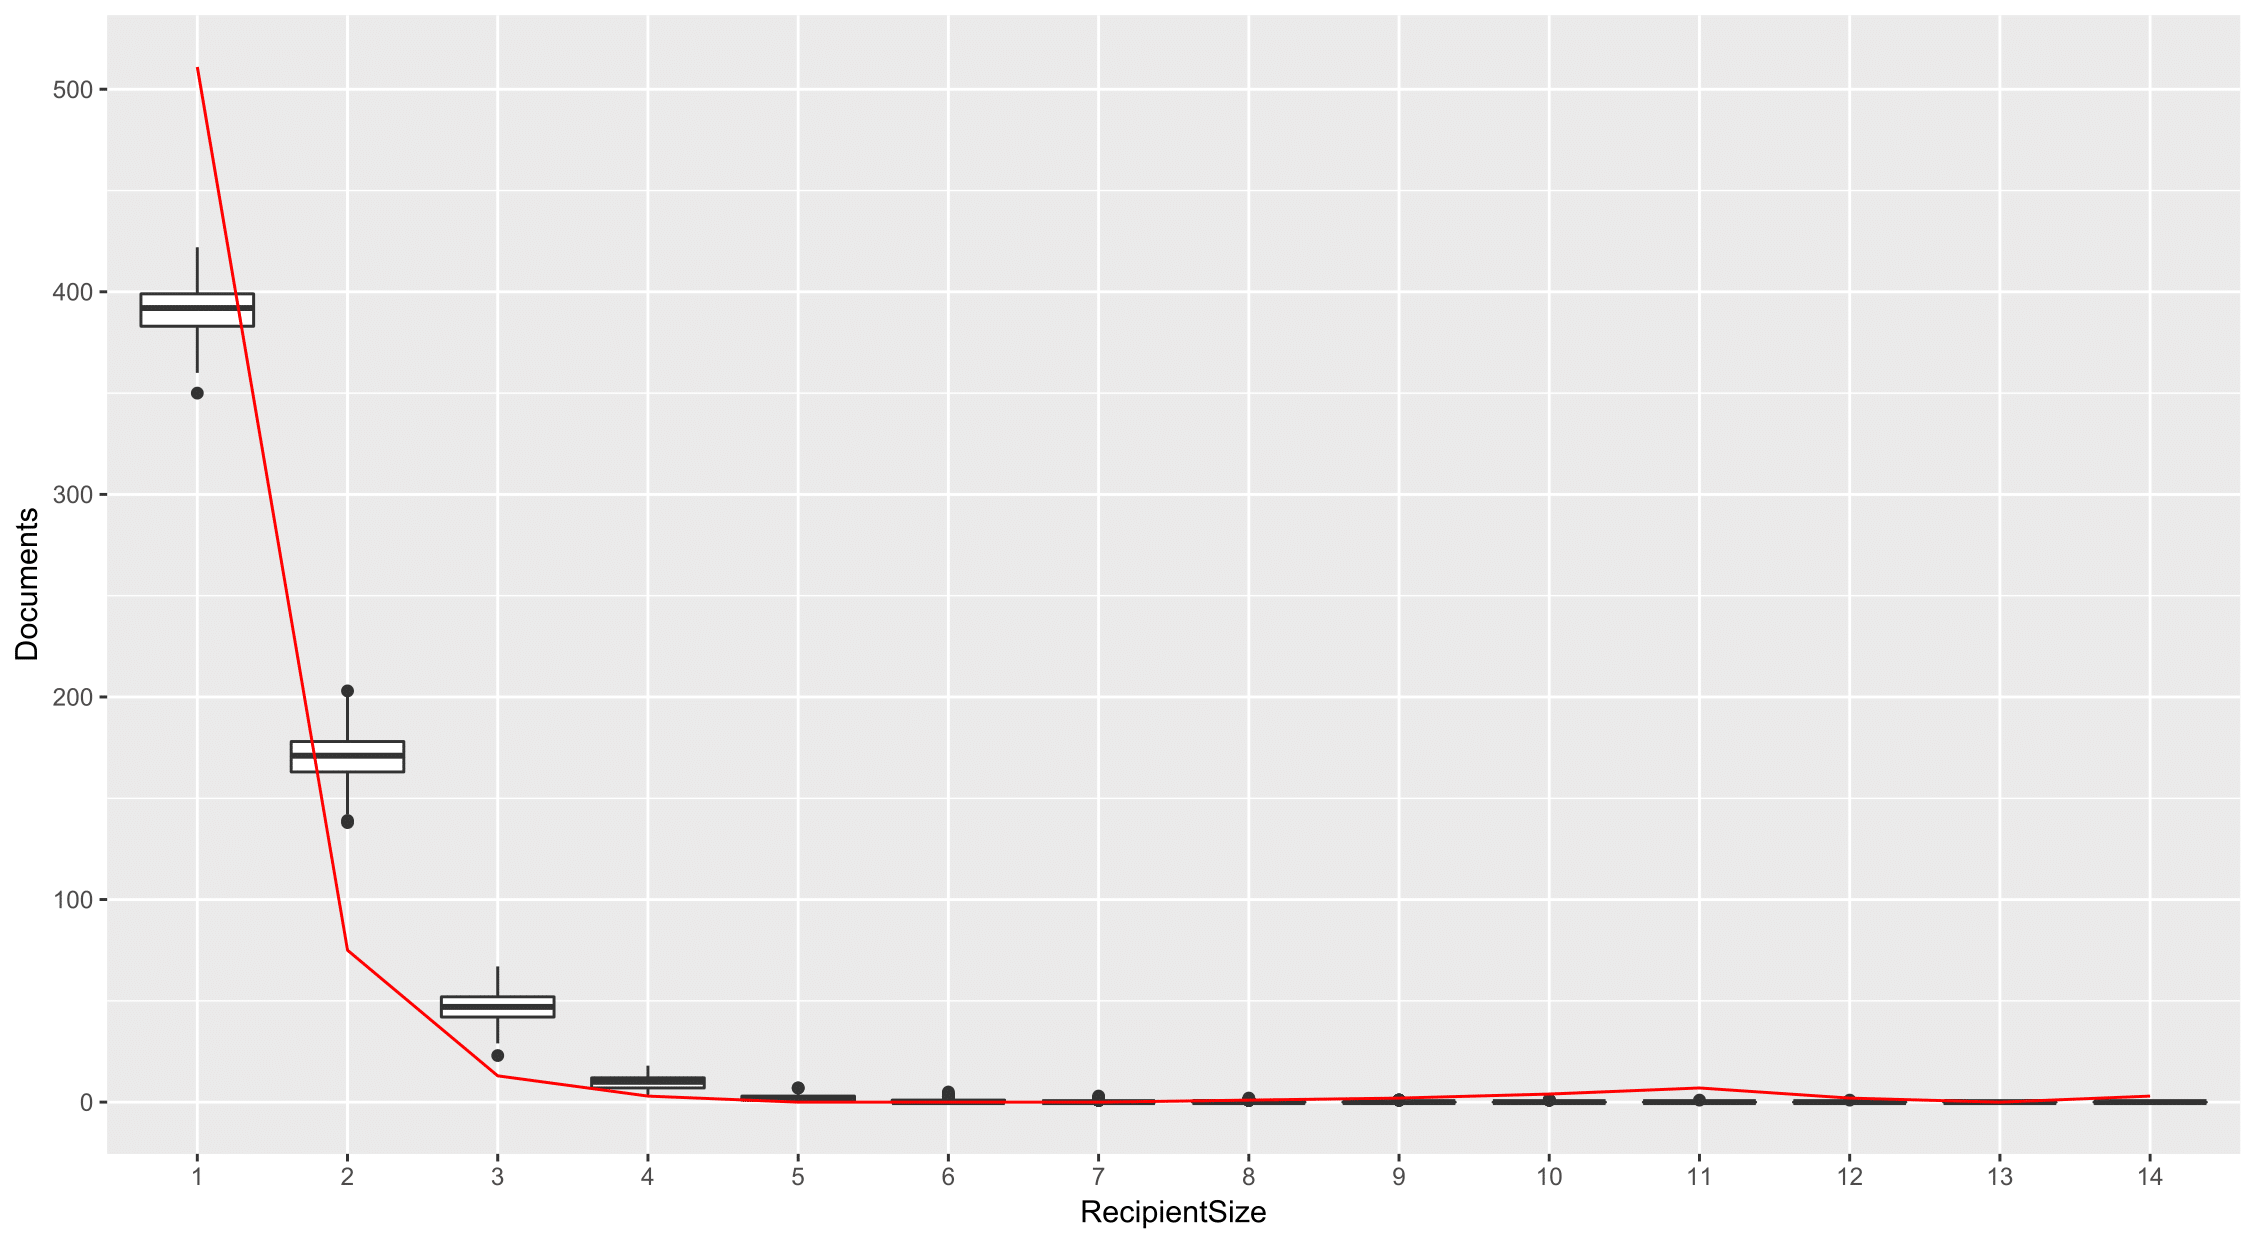
\includegraphics[width=0.495\textwidth]{plots_paper/recipientsize_exp-1.png}	
 		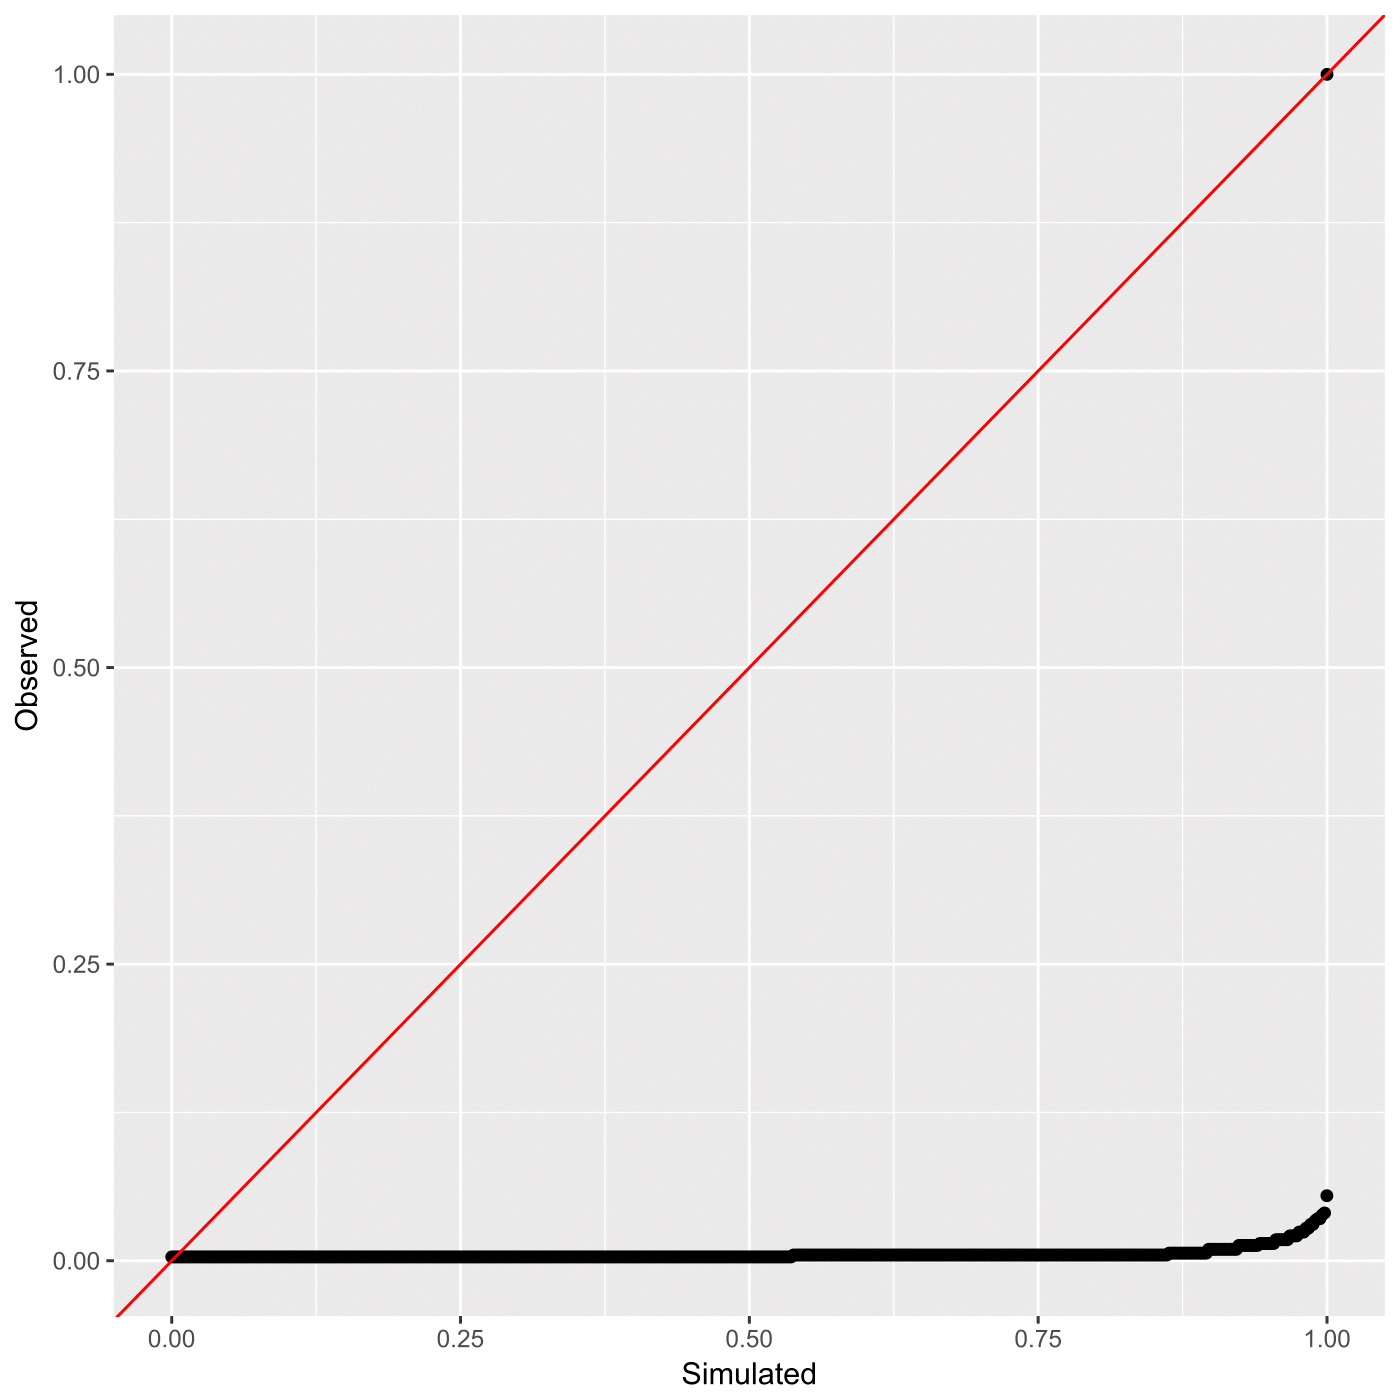
\includegraphics[width=0.31\textwidth]{plots_paper/timepp_exp-1.png}
 		\caption {PPC results from exponential distribution: outdegree distribution (\textit{upper left}), indegree distribution (\textit{upper right}), recipient size distribution (\textit{lower left}), and time-increments probability-probability (PP) plot  (\textit{lower right}). Red lines in the first three plot depict the observed statistics, and the red line in the last plot is the diagonal line connecting $(0, 0)$ and $(1, 1)$.}
 		\label{figure:PPCexp}
 	\end{figure}
	\end{appendices}
\end{document}